\documentclass{VUMIFPSkursinis}
\usepackage{algorithmicx}
\usepackage{algorithm}
\usepackage{algpseudocode}
\usepackage{amsfonts}
\usepackage{amsmath}
\usepackage{bm}
\usepackage{caption}
\usepackage{color}
\usepackage{float}
\usepackage{graphicx}
\usepackage{listings}
\usepackage{subfig}
\usepackage{wrapfig}
\usepackage{sectsty}
\usepackage{enumerate}
\usepackage{longtable}
\usepackage[export]{adjustbox}
\usepackage{rotating}
\usepackage{hhline}
\usepackage{multirow}
\usepackage{tabularx}
\usepackage{array}
\usepackage{booktabs,calc}
\usepackage{tabularx,colortbl}
\usepackage[table]{xcolor}  
\usepackage{longtable}  

\usepackage{enumitem}
%PAKEISTA, tarpai tarp sąrašo elementų
\setitemize{noitemsep,topsep=0pt,parsep=0pt,partopsep=0pt}
\setenumerate{noitemsep,topsep=0pt,parsep=0pt,partopsep=0pt}
\allsectionsfont{\centering}
% Titulinio aprašas
\university{Vilniaus universitetas}
\faculty{Matematikos ir informatikos fakultetas}
\department{Programų sistemų katedra}
\papertype{Programų sistemų inžinerijos I-III laboratoriniai darbai}
\title{Socialinis Vilniaus universiteto tinklalapis}
\titleineng{SocialVU}
\status{2 kurso 4 grupės studentai}
\author{Andrejus Voitovas}
\secondauthor{Eglė Puodžiūnaitė}
\thirdauthor{Kasparas Kralikas}
\fourthauthor{Ieva Vizgirdaitė} % Pridėti antrą autorių
\supervisor{asist. dr. Vytautas Valaitis}
\date{Vilnius – \the\year}

% Nustatymai
% \setmainfont{Palemonas}   % Pakeisti teksto šriftą į Palemonas (turi būti įdiegtas sistemoje)
\bibliography{bibliografija}

\begin{document}
% PAKEISTA
\maketitle
\cleardoublepage\pagenumbering{arabic}
\setcounter{page}{2}
\sectionnonum{ANOTACIJA}
PATAISYT!!!!!!!!!!!!!!!!!!!!!!!!!!!!!
Šiame dokumente pateikiama dalykinės srities analizė. Išorinėje verslo proceso analizėje identifikuojamos pagrindinės grėsmės ir galimybės. Vidinėje verslo proceso analizėje nustatomos verslo stiprybės ir silpnybės, kylančios iš paties verslo proceso. Be to dokumente pateikiamos verslo tobulinimo strategijos, nagrinėjamos galimybės įgyvendinti sistemą tiek techniniu tiek ir ekonominiu požiūriu.\\
Rašant šį dokumentą buvo naudojamasi:
\begin{enumerate}
	\item dr. Vytauto Valaičio internetinis puslapiu (https://klevas.mif.vu.lt/~valaitis/) 
	\item doc., dr. Karolio Petrausko iternetiniu puslapiu (http://klevas.mif.vu.lt/~karolis/) 
	\item Latex programa
	\item lab. asst. Jono Brusoko parengtais kursinio darbo šablonais (https://gitlab.com/JohnLogic/SE-course-work-template)
	
\end{enumerate}
\newpage
%TURINYS
\tableofcontents

\sectionnonum{ĮVADAS}
Socialinis VU tinklapis kuriamas siekiant supaprastinti informacijos prieinamumą visai fakulteto bendruomenei. Tinklapis suteikia galimybę patogiai dalintis informacija, susisiekti su dėstytojais/studentais. Fakultetui suteikiama galimybė platesniu mastu platinti su fakultetu susijusias naujienas. \\
Dokumente pateikiamas pagrindinis programos funkcionalumas ir tam tikri ribojimai jos
kūrimui. Pasitelkiant ICONIX metodą sudaromi užduočių scenarijai, apibrėžiamos pagrindinės
kuriamos sistemos esybės, sudaromas struktūrinis dalykinės srities modelis. Šis dokumentas
padeda toliau projektuoti ir nuspręsti, kaip sistema turėtų būti įgyvendinta.\\
\textbf{Temos aktualumas} \\
Šiuo metu, dauguma informacijos skirtos studentams yra išdėstyta padrikai, todėl nuspręsta sudėti visą informaciją į vieną vietą. Yra atskiras universiteto naujienų puslapis, kiekvienas dėstytojas turi savo asmenininį puslapį bei el. paštą, tačiau šią informaciją studentams surasti yra itin komplikuota, o dėstytojams pateikti informaciją savo puslapiuose yra nepatogu.\\
\textbf{Dalykinė sritis}\\
Socialinis Vilniaus Universiteto tinklapis.\\
 \textbf{Probleminė sritis}\\
Socialinis VU tinklapis suteiktų galimybę greitai ir paprastai pasiekti dėstytojų pateiktą informaciją. Taip pat susisiekti su pačiais dėstytojais, sekti aktualias fakulteto naujienas, renginius. Pagrindinis šio produkto išskirtinumas - greitai ir patogiai pasiekiama informacija, todėl itin svarbi informacija pasieks galutinius vartotojus.\\
 \textbf{Naudoti dokumentai}\\
 Dokumentas parengtas pagal kursinio darbo reikalavimus naudotojant Latex programą ir jau
sukurtus šabonus.
\\
 \textbf{Darbo pagrindas} \\ 
Dokumentas parengtas kaip Programų sistemų inžinerijos I-III laboratorinis darbas.
\newpage
\section{KURIAMO VERSLO PROCESO ANALIZĖ}
\subsection{VERSLO PROCESO APRAŠAS}

Ši sistema turi trijų tipų vartotojus - studentus, dėstytojus bei administratorius. Visų pirma, prisijungus prie sistemos vartotojas yra nukreipiamas į pagrindinį sistemos puslapį.

Studentai pagrindiniame sistemos puslapyje gali matyti universiteto naujienas, artėjančius renginius. Taip pat čia yra prieinamos nuorodos į kitas esmines sistemos dalis - dėstytojų puslapius, konspektų dalinimosi platformą, D.U.K. skiltį bei žinučių sistemą. Kiekvienas studentas turi prieigą prie savo dėstytojų asmeninių puslapių. Čia galima rasti informaciją apie dėstomus dalykus, jų medžiagą, bei artėjančius atsiskaitymus. Žinučių sistemoje studentas įgalinamas komunikuoti tiek su kitais studentais, tiek su dėstytojais, taip pat žinučių pavidalu gaunami priminimai apie artėjančius renginius ar atsiskaitymus. Konspektų dalinimosi platformoje studentas gali peržiūrėti kitų studentų įkeltus konspektus, juos įsigyti. Taip pat studentas gali peržiūrėti jau įsigytus konspektus, juos peržiūrėti naršyklėje arba atsisiųsti į savo kompiuterį ar mobilųjį įrenginį. Galiausiai, studentas gali į sistemą patalpinti ir savuosius konspektus, nurodydamas konspektų paskirtį bei jų kainą. D.U.K. skiltyje studentai gali rasti naudingą informaciją įvairia tematika, taip pat atsakymus į didžiąją dalį iškylančių klausimų.

Dėstytojai pagrindiniame sistemos puslapyje taip pat gali matyti universiteto naujienas, artėjančius renginius. Čia jiems yra prieinamos ir nuorodos į esmines, dėstytojams skirtas, sistemos dalis - naujienų, renginių bei D.U.K. skilties redagavimą, žinučių sistemą bei asmeninio puslapio administravimo erdvę. Naujienų redagavimo skiltyje dėstytojai gali patalpinti informaciją apie įvairias aktualijas, taip pat redaguoti senesnius įrašus, juos ištrinti. Renginių redagavimo skiltyje dėstytojai gali kurti naujus renginius, siųsti kvietimus žinučių pavidalu, peržiūrėti senesnius renginius, juos ištrinti. D.U.K. skilties redagavimo aplinkoje dėstytojai gali peržiūrėti esamus klausimus ir atsakymus, redaguoti jų turinį, pridėti naujus klausimus. Žinučių sistemoje dėstytojai gali matyti gautas bei išsiųstas žinutes, gali siųsti žinutes studentams, kitiems dėstytojams, čia gauna priminimus apie artėjančius svarbius įvykius (renginius, atsiskaitymus). Asmeninio puslapio administravimo erdvėje dėstytojai gali talpinti informaciją apie savo dėstomus dalykus, šią informaciją paslėpti nuo studentų ar padaryti ją prieinamą tik šiuo metu tam tikrą dėstomą dalyką turintiems studentams. Taip pat dėstytojas gali kurti papildomus puslapius, prieinamus iš pagrindinio dėstytojo asmeninio puslapio.

Visą sistemos darbą prižiūri sistemos administratorius. Jis atsakingas už vartotojų registracijos patvirtinimą, vartotojų pašalinimą ar pridėjimą.

\newpage
\subsection{IŠORINĖ VERSLO PROCESO ANALIZĖ}
Išorinė analizės metu išsiaiškinami ištekliai
reikalingi pradėti verslą, išryškinamos kuriamo verslo grėsmės ir
problemos, kuriami tinklalapio teikiami rezultatai ir išanalizuojama rinkoje esanti situacija. Nustačius rinkoje esančius ir potencialius konkurentus išanalizuojamos
neišnaudotos galimybės bei įvertinama situacija.

\ref{ieigos}, \ref{iseigos}, \ref{ivaizdis} ir \ref{reguliavimas} lentelėse pateikiami įeigos, išeigos, reguliavimo ir įvaizdžio svarbiausi vertinimo kriteriai,
jų matavimo vienetai. Nustatoma kritinė vertė, esama vertė ir siekiama vertė. Tai padeda
nustatyti, ar tam tikras vertinimo kriterijus atitinka normas.
\subsubsection{Įeigos}
\begin{enumerate}
	\item Studentai
	\item Dėstytojai
	\item Administratorius
	\item Duomenų bazė
	\item Serveris
\end{enumerate}
\begin{table}[H]
	\centering
	\caption{Įeigos}
	\resizebox{\textwidth}{!}{\begin{tabular}{|c|c|c|c|} \hline
			Vertinimo kriterijus & Vertinimo matas & Siekiama vertė & Kritinė vertė \\
			\hline
			Studentai & Kiekis studentų, naudojančių socialVU tinklalapį & 21281 & 10000 \\
			\hline
			Dėstytojai & Kiekis dėstytojų, naudojančių socialVU tinklalapį & 2890 & 1500 \\
			\hline
			Administratorius & Pašalintų naudotojų skaičius per
			mėnesį & 0 & 30 \\
			\hline
			Duomenų bazė & Talpa GB & 50 & 10 \\
			\hline
			Serveris & Vidutinis užklausos apdorojimo laikas sekundėmis & 1 & 5 \\
			\hline
	\end{tabular}}
	\label{ieigos}
\end{table}
\subsubsection{Išeigos}
\begin{enumerate}
	\item Studentai, radę visą reikiamą informaciją
	\item Dėstytojai, pateikę visą norimą informaciją
\end{enumerate}
\begin{table}[H]
	\centering
	\caption{Išeigos}
	{\begin{tabular}{|c|c|c|c|} \hline
			Vertinimo kriterijus & Vertinimo matas & Siekiama vertė & Kritinė vertė \\
			\hline
			Studentai, radę visą reikiamą informaciją & Kiekis per mėnesį \% & 100 & 50 \\
			\hline
			Dėstytojai, pateikę visą norimą informaciją & Kiekis per mėnesį \% & 100 & 50 \\
			\hline
	\end{tabular}}
	\label{iseigos}
\end{table}
	\subsubsection{Įvaizdis}
\begin{enumerate}
	\item Dėstytojų bei studentų atsiliepimai
	\item Sistemos žinomumas
\end{enumerate}
\begin{table}[H]
	\centering
	\caption{Įvaizdis}
	{\begin{tabular}{|p{5cm}|p{6,5cm}|p{2cm}|p{2cm}|}\hline
			Vertinimo kriterijus & Vertinimo matas & Siekiama vertė & Kritinė vertė \\
			\hline
			Dėstytojų bei studentų atsiliepimai & Teigiamų atsiliepimų \% nuo visų atsiliepimų & 90 & 50 \\
			\hline
			Sistemos žinomumas & Vilniaus universiteto studentų \% žinančių šį tinklalapį & 100 & 50 \\
			\hline
	\end{tabular}}
	\label{ivaizdis}
\end{table}
	\subsubsection{Reguliavimas}
\begin{enumerate}
	\item Asmens duomenų teisinės apsaugos įstatymas
	\item Darbo kodeksas
\end{enumerate}
\begin{table}[H]
	\centering
	\caption{Įvaizdis}
	{\begin{tabular}{|p{5cm}|p{6,5cm}|p{2cm}|p{2cm}|} \hline
			Vertinimo kriterijus & Vertinimo matas & Siekiama vertė & Kritinė vertė \\
			\hline
			Asmens duomenų teisinės apsaugos įstatymas & Pažeidimų skaičius & 0 & 0 \\
			\hline
			Darbo kodeksas & Viršytas darbo laikas (kartais per metus) & 0 & 0 \\
			\hline
	\end{tabular}}
	\label{reguliavimas}
\end{table}
\subsubsection{Grėsmės}
Kuriamas verslas yra priklausomas nuo dviejų pagrindinių įvesčių - dėstytojų ir studentų. Jų skaičius ir aktyvumas lemia kuriamos programos sėkmę. Rinkoje jau egzistuoja nemažai socialinių tinklų, kuriuos naudoja dauguma studentų (Facebook, Instagram, Linkedin, Twitter ir t.t.) be to dauguma dėstytojų yra ipratę skelbti visą informaciją savo sukurtuose puslapiuose arba bando integruoti informaciją į Vilniaus universiteto virtualią mokymosi aplinką, todėl konkurencija yra gana didelė. Kuo daugiau dėstytojų pradės naudoti mūsų sukurtą platformą, tuo daugiau studentų taip pat privalės naudoti šį tinklalapį, nes tik ten galės rasti jiems reikiamą informaciją. Sėkmingam kuriamo verslo proceso egzistavimui turi įtakos reitingų ir atsiliepimų skaičius bei kokybė, tačiau visų pirma reikia užtikrinti, jog dauguma studentų bei dėstytojų išbandytų mūsų sukurtą sistemą bei ją įvertintų.
\subsubsection{Neišnaudotos galimybės}
Rinkoje jau egzistuojančios Vilniaus universiteto platformos turi trūkumų (dauguma dėstytojų skelbia informaciją skirtinguose puslapiuose, todėl studentams sunku juos surasti, ne visada yra galimybė susisiekti su dėstytojais, dauguma konspektų nėra lengvai pasiekiami visiems studentams), todėl kuriama sistema gali juos išnaudoti ir pasiūlyti studentams visą reikiamą informaciją rasti vienoje vietoje. Sistema suteiks galimybę išsiųsti laišką dėstytojui bei rasti visą paskelbtą dėstytojo informaciją vienoje vietoje, studentai galės matyti naujausią informaciją bei terminus iki kada turi atlikti tam tikras užduotis. Be to vienoje vietoje galės rasti visus reikiamus konpektus bei pasidalinti turimais konspektais su kitais studentais ir taip padėti mokytis kitiems.
\newpage
\newpage
\subsection{VIDINĖ VERSLO PROCESO ANALIZĖ}
Toliau pateikiama keliais aspektais atlikta vidinė verslo proceso analizė, kuria siekiama
nustatyti nagrinėjamo verslo stiprybes ir silpnybes, kylančias iš verslo proceso.

\subsubsection{Sąvokos}
Šiame skyriuje pateikiami specifiniai mūsų projekte naudotų žodžių paaiškinimai. \\
\textbf{Sistema} – fakulteto vidinis socialinis tinklas, dokumente vadinamas „SocialVU“. \\
\textbf{Studentas} – vartotojas, kuris turim ribotas galimybes turinio valdymo atžvilgiu.\\
\textbf{Dėstytojas} – vartotojas, kuris turi galimybę redaguoti visą socialinio tinklo turinį.\\
\textbf{Administratorius} – vartotojas, kuris turi galimybę redaguoti visą socialinio tinklo turinį, išskyrus dėstytojus.

\subsubsection{Dalykinės srities statinė struktūra}
 Toliau pateikiama dalykinės srities statinės struktūros UML diagrama. Joje matomos pagrindinės esybės bei jų tarpusavio sąveika. Klientai yra trijų tipų: studentai, dėstytojai ir administratoriai (dėstytojai bei administratoriai skiriasi turinio redagavimo teisėmis). Studentams, administratoriams ir dėstytojams registruotis nereikia, nes visa vartotojų duomenų bazė bus imama iš bendros VU vartotojų duomenų bazės. Vartotojui tereikia autentifikuoti save - tokiu būdu, priklausomai nuo užimamų pareigų, jam bus suteiktos teisės prie numatyto turinio. Studentai gali tik skaityti tokius puslapius kaip "Dėstytojai", "Naujienos", "Renginiai", "D.U.K", "Konspektai". Tuo tarpu dėstytojai skiltyje "Naujienos" gali parašyti naujieną. Be to, jiems suteikta prieiga prie jų profilio, kur turi teisę redaguoti savo asmeninį puslapį, siųsti bei gauti žinutes, pridėti organizuojamą renginį. Administratoriumi gali būti fakulteto paskirtas žmogus, atsakingas už tikslingo turinio formavimą vidiniame socialiniame tinkle arba VU Studentų atstovybės narys, kuris turi teisę redaguoti visą turinį. Tačiau joks administratorius negali redaguoti dėstytojo sukurto turinio.\\

\begin{figure}[H]
\centering
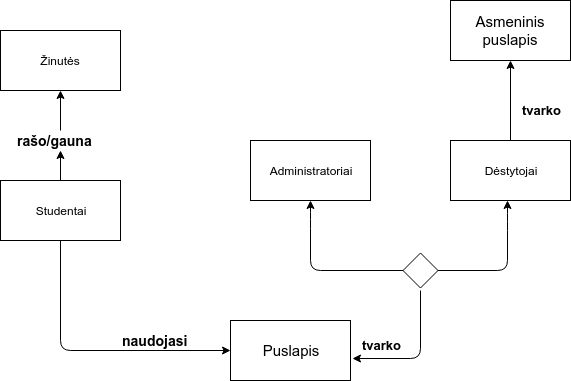
\includegraphics[width=\linewidth]{img/dalykine.png}
\label{fig:dalykine}
\caption{Dalykinė srities UML diagrama}
\end{figure}

\subsubsection{Užduotys}
\begin{figure}[H]
\centering
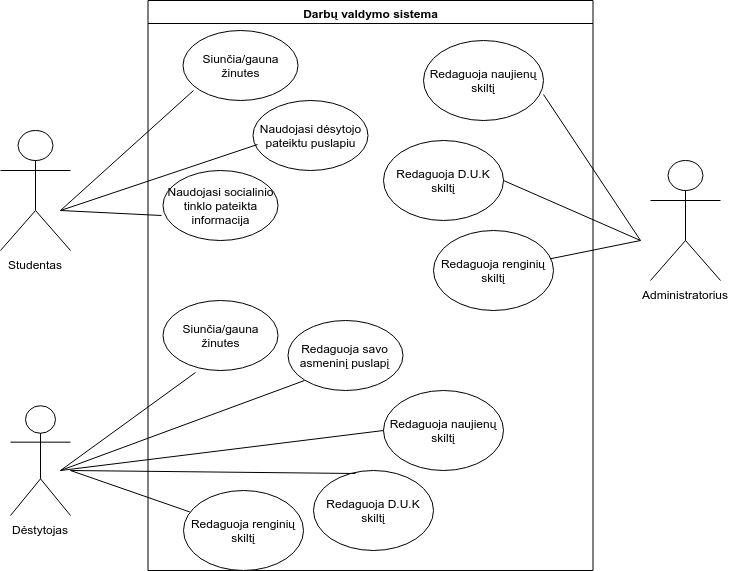
\includegraphics[width=\linewidth]{img/DVS.png}
\caption{Užduočių veiklos UML diagrama}
\label{fig:dvs}
\end{figure}
Užduočių sąrašas pagal \ref{fig:dvs} pav.:\\
\textbf{Užduotis:} sukurti naujieną. \\
\textbf{Tikslas:} publikuoti naujieną, kuri būtų įdomi.\\
\textbf{Trigeris:} administratoriaus arba dėstytojo kuriama naujiena tituliniui. \\
\textbf{Prioritetas:} aukštas. \\
\textbf{„Prieš” sąlygos:} naujiena bus skaitoma.\\
\textbf{Sėkmingos baigties „po” sąlyga:} naujiena perskaitoma ir įsisavinama nauja informacija. \\
\textbf{Nesėkmingos baigties sąlyga:} naujiena visiškai nėra skaitoma. \\
\textbf{Pirminis agentas:} administratorius. \\
\textbf{Antriniai agentai:} studentas. \\
\\
\textbf{Užduotis:} redaguoti puslapį. \\
\textbf{Tikslas:} redaguoti dėstytojo puslapį.\\
\textbf{Trigeris:} prisijungęs dėstytojas gali redaguoti puslapį. \\
\textbf{Prioritetas:} aukštas. \\
\textbf{„Prieš” sąlygos:} dėstytojas patogiai talpina informaciją.\\
\textbf{Sėkmingos baigties „po” sąlyga:} dėstytojo informacija sudėliota pagal šabloną ir patogi naudojimuisi. \\
\textbf{Nesėkmingos baigties sąlyga:} dėstytojas nesudaro savo puslapio. \\
\textbf{Pirminis agentas:} dėstytojas. \\
\textbf{Antriniai agentai:} studentas. \\
\\
\textbf{Užduotis:} sukurti renginį. \\
\textbf{Tikslas:} publikuoti renginį, kuris būtų naudingas.\\
\textbf{Trigeris:} administratoriaus arba dėstytojo sukurtas renginys atsiranda puslapyje. \\
\textbf{Prioritetas:} aukštas. \\
\textbf{„Prieš” sąlygos:} renginį aplankys daug žmonių.\\
\textbf{Sėkmingos baigties „po” sąlyga:} renginys pateisino savo lūkesčius. \\
\textbf{Nesėkmingos baigties sąlyga:} apie renginį studentai sužinojo ne iš socialinio tinklo. \\
\textbf{Pirminis agentas:} administratorius. \\
\textbf{Antriniai agentai:} studentas. \\
\\
\textbf{Užduotis:} parašyti žinutę. \\
\textbf{Tikslas:} parašyti žinutę tiesiai vartotojui.\\
\textbf{Trigeris:} studentas, paspaudęs ant dėstytojo, gali parašyti jam žinutę. \\
\textbf{Prioritetas:} aukštas. \\
\textbf{„Prieš” sąlygos:} vartotojas gaus žinutę.\\
\textbf{Sėkmingos baigties „po” sąlyga:} vartotojai patogiai komunikuos tarpusavy. \\
\textbf{Nesėkmingos baigties sąlyga:} žinutė liks neperskaityta. \\
\textbf{Pirminis agentas:} studentas. \\
\textbf{Antriniai agentai:} administratorius.\\
\\
\textbf{Užduotis:} apsilankyti asmeniniame puslapyje. \\
\textbf{Tikslas:} pasiekti dėsytotojo asmeninį puslapį.\\
\textbf{Trigeris:} studentų apsilankymas dėstytojų profilyje. \\
\textbf{Prioritetas:} aukštas. \\
\textbf{„Prieš” sąlygos:} vartotojai lankysis dėstytojų puslapiuose per socialinį tinklą.\\
\textbf{Sėkmingos baigties „po” sąlyga:} vartotojams bus patogu pasiekti puslapį ir sužinoti informaciją. \\
\textbf{Nesėkmingos baigties sąlyga:} vartotojai toliau ieškos puslapių naudojantis "Google". \\
\textbf{Pirminis agentas:} studentas. \\
\textbf{Antriniai agentai:} administratorius.

\subsubsection{Užduočių vykdymo scenarijai}
\ref{fig:klasiu} pav. paveikslėlyje pavaizduota esybių diagrama. Pateikiamos pagrindinės dalykinės srities esybės, pavaizduoti ryšiai tarp jų.
\begin{figure}[H]
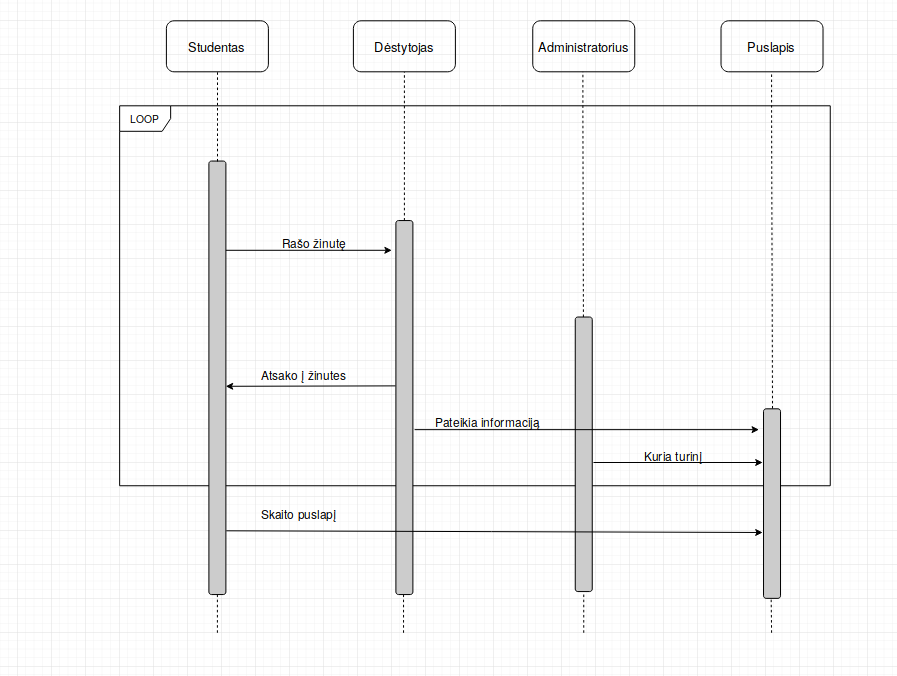
\includegraphics[width=\linewidth]{img/bendra-uml.png}
\caption{Klasių diagrama}
\label{fig:klasiu}
\end{figure}
\ref{fig:klasiu} pav. vaizuduojamas socialinio tinklo naudojimosi modelis. Studentas gali rašyti dėstytojui žinutę, o dėstytojas jam gali atsakyti. Taip pat studentas skaito puslapį, kurį pats dėstytojas ir sukūrė. Administratorius kuria turinį, į kurį įeina: renginiai, naujienos, D.U.K.
\subsubsection{Dalykinės srities dinaminė struktūra}
Studentas:
\begin{figure}[H]
\centering
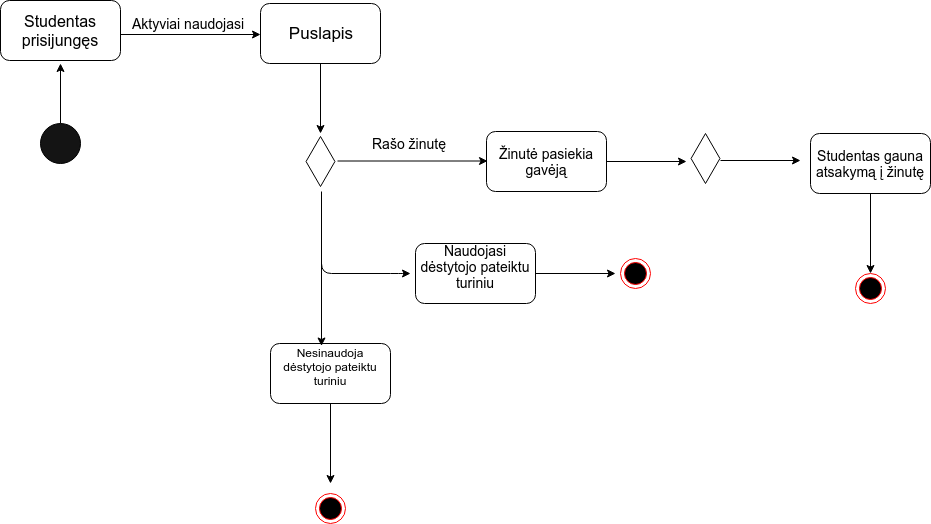
\includegraphics[width=\linewidth]{img/studentas.png}
\caption{Studento UML klasių diagrama}
\label{fig:studentu}
\end{figure}
\ref{fig:studentu} pav. Prisijungęs studentas turi galimybę matyti bendrą turinį. Vėliau gali parašyti žinutę dėstytojui arba naudojasi dėstytojo pateiktu turiniu. Jie tarpusavyje gali komunikuoti socialinio tinklo pagalba, nenaudojant trečiųjų šalių servisų.\\
Dėstytojas: \\
\begin{figure}[H]
\centering
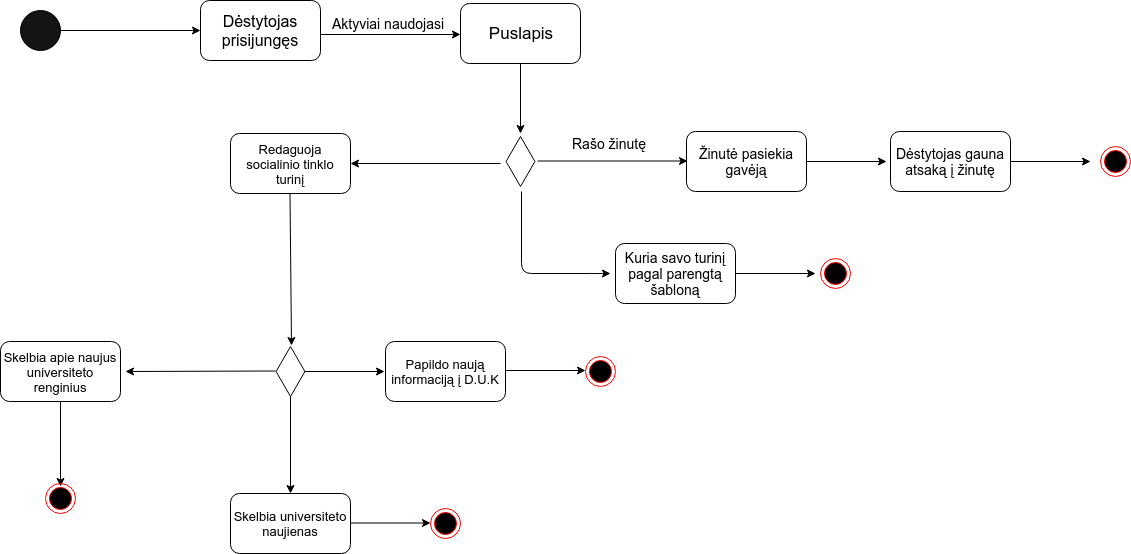
\includegraphics[width=\linewidth]{img/destytojas.png}
\caption{Dėstytojo UML klasių diagrama}
\label{fig:destytoju}
\end{figure}
\ref{fig:destytoju} pav. Prisijungęs dėstytojas turi galimybę redaguoti savo puslapio turinį, pagal iš anksto paruoštą šabloną. Dar turi galimybę rašyti bei atsakyti į studentų gautas žinutes. Naujienų rašymas, renginių kūrimas, D.U.K skilties papildymas irgi įeina į aukščiau aprašomo vartotojo galimybes.\\
Administratorius: \\
\begin{figure}[H]
\centering
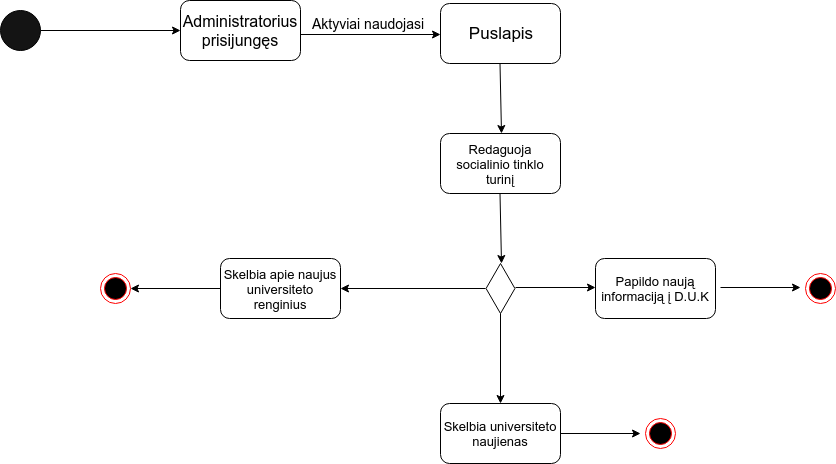
\includegraphics[width=\linewidth]{img/administratorius.png}
\caption{Administratoriaus UML klasių diagrama}
\label{fig:administratoriu}
\end{figure}
\ref{fig:administratoriu} pav. Prisijungęs administratorius, tai žmogus, kuris atsakingas už bendrą socialinio tinklo turinį, į kurį neįeina dėstytojų puslapių redagavimas. Administratorius gali kurti bei redaguoti tik naujienų, D.U.K ir renginių skiltis.\\

\newpage
\subsection{ĮGYVENDINAMUMO IR NAUDOS ANALIZĖ}
Šiame skyriuje pateikiama informacija, kuri padeda nustatyti, ar darbų valdymo sistemą
įmanoma sukurti, kokią konkrečią naudą ji duos, kokios problemos gali kilti ir kaip jos bus sprendžiamos.

\subsubsection{Operacinis įgyvendinamumas}
Šiame skyriuje pateikiami galimi trukdžiai, kurie gali kilti naudantis sistema, bei pateikiami
galimi jų sprendimo būdai.\\
\\
\textbf{Problema:}
Pasikartojančių konspektų bei kitos dalykinės informacijos perteklius.
\\
\textbf{Sprendimo būdas:}
Studentų atstovybės paskirtas žmogus nuolat tikrina konspektų naudą arba prieš įkeliant konspektą, studentas turi gauti patvirtinimą.\\
\\
\textbf{Problema:}
Universiteto bendruomenė nesinaudoja mūsų sistema t.y. dėstytojai toliau pateikia savo asmeninius puslapius per senąsias nuorodas, studentai ieško informacijos kituose šaltiniuose.
\\
\textbf{Sprendimo būdas:}
Prašyti studentų atstovybės pagalbos, kad informuotų bendruomenę apie naudojimosi galimybes bei teikiamą naudą.\\
\\
\textbf{Problema:}
internetinis puslapis dažnai patiria sistemos perkrovą.
\\
\textbf{Sprendimo būdas:}
Naudoti galingesnius serverius, kurie sugeba apdoroti didesnius vartotojų srautus.

\subsubsection{Techninis įgyvendinamumas}
Šiuo metu jau egzistuoja atskiri Vilniaus universiteto informacinės sistemos komponentai (el. paštas, VU informacinė sistema, fakultetų puslapiai, dėstytojų asmeniniai puslapiai). Mūsų kuriama sistema visus šiuos komponentus apjungtų į vieną bendrą sistemą. Vienintelis reikalavimas vartotojams - interneto prieiga.

\subsubsection{Ekonominis įgyvendinamumas}
\textbf{Išlaidos}

Prognozuojama sistemos sukūrimo kaina - 8960€. Daroma prielaida, jog sistemos sukūrimas truks 16 savaičių, jei prie sistemos kūrimo puse etato dirbs keturių žmonių komanda (kiekvienam asmeniniui mokamas 7€/h atlyginimas).

Sistemos palaikymo kaina - 2184€/mėn. Daroma prielaida, jog sistemą prižiūri du pilnu etatu už 6€/h darbo užmokestį dirbantys sistemos administratoriai, serverio nuoma kainuoja 139€/mėn, o reklamos išlaidos sudaro 125€ per mėnesį.

Kitos išlaidos pateikiamos sekančioje lentelėje.

\begin{table}[H]
	\centering
	\caption{Išlaidos reikalingos sistemos sukūrimui ir palaikymui}
    {\begin{tabular}{|c|c|c|c|} \hline
			Išlaidos & Kaina  \\
			\hline
			Sistemos sukūrimas & 8960€\\
			\hline
			Domeno registracija & 10€  \\
			\hline
			SSL sertifikatas & 155.55€ \\
			\hline
			Serverio nuoma & 139€ mėnesiui \\
			\hline
			Administratoriai & 1920€ mėnesiui \\
			\hline
			Reklama & 125€ mėnesiui \\
			\hline
	\end{tabular}}
\end{table}

\textbf{Pajamos}

Pagrindinis kuriamos sistemos pajamų šaltinis - konspektų dalinimosi platforma. Darant prielaidą, jog iš šiuo metu esančių 20000 Vilniaus universiteto studentų 3 procentai jų nuspręs patalpinti konspektus į konspektų dalinimosi platformą pardavimui už vidutinę 5€ kainą (20 procentų pelno lieka platformos savininkams) ir kiekvieno studento patalpintas egzempliorius bus nuperkamas vidutiniškai kartą į savaitę, metinės sistemos pajamos turėtų siekti apie 31284€.

\textbf{Pelnas/nuostolis}

Metinės sistemos palaikymo išlaidos turėtų sudaryti 26208€. Atsižvelgiant į sukūrimo kaštus, sistema turėtų pradėti generuoti pelną po 1.76 metų. Tikėtinas metinis pelnas - 5076€.

\subsubsection{Juridinis įgyvendinamumas}

 Sistema nepažeis Lietuvos respublikos įstatymų, Europos Sąjungos direktyvų bei Lietuvos respublikos konstitucijos. Vartotojų duomenys bus saugomi, tvarkomi bei perduodami naudojantis užšifruota sąsaja laikantis asmenų duomenų apsaugos įstatymo. Vartotojų talpinamų konspektų autorinės teisės bus saugomos remiantis Lietuvos Respublikos autorių teisių ir gretutinių teisių įstatymu. 

\newpage

\subsection{SISTEMOS NAUDOJIMO SCENARIJUS}
Šiame skyriuje aprašomas socialinio tinklalapio naudojimo scenarijus.
\subsubsection{Scenarijus}
Šiame skyriuje pateikiami pagrindinių funkcijų modeliai, kurie parodo, kaip pagrindiniai sistemos agentai, šiuo atveju studentai, dėstytojai ir administratoriai, naudosis sistema. Tam naudojamos UML sekų diagramos.
\begingroup
\begin{figure}[H]
\centering
\includegraphics[width=\linewidth]{img/uzdNaujiena.png}
\caption{Užduoties įrašyti naujieną modelis}
\label{fig:rnaujiena}
\end{figure}
\setlength{\parindent}{0pt}\textbf{Užduotis: } Įrašyti naujieną\\
\textbf{Tikslas: } paskelbti aktualią naujieną.\\
\textbf{Pirminis agentas: } dėstytojas.\\
\textbf{"Prieš" sąlyga: } naudotojas yra prisijungęs tinklalapyje, dėstytojo aplinkoje.\\
\textbf{"Po" sąlyga: } aktuali naujiena yra patalpinta tinklalapyje.\\
\textbf{Scenarijus: } naudotojas, prisijungęs kaip dėstytojas, pasirenka naujienos sukūrimo puslapį ir gražintoje formoje suveda norimą paskelbti informaciją bei pasirenka, kam ši naujiena yra skirta(studentams, dėstytojams, visiems). Jeigu naujiena neatitinka formato ar yra tuščia, sistema įspėja dėstytoją ir leidžia pakeisti duomenis. Jeigu duomenys atitinka formatą, dėstytojas yra informuojamas apie sėkmingą naujienos patalpinimą pagrindiniame puslapyje.
\begin{figure}[H]
\centering
\includegraphics[width=\linewidth]{img/uzdSiustiZinute.png}
\caption{Užduoties siųsti žinutę modelis}
\label{fig:zinute}
\end{figure}
\textbf{Užduotis: } studentui išsiųsti žinutę dėstytojui\\
\textbf{Tikslas: } studento išsiųsta žinutė pasiekia dėstytoją\\
\textbf{Pirminis agentas: } studentas\\
\textbf{"Prieš" sąlyga: } naudotojas yra prisijungęs tinklalapyje, studento aplinkoje.\\
\textbf{"Po" sąlyga: } studento žinutė yra išsiųsta\\
\textbf{Scenarijus: } naudotojas, prisijungęs kaip studentas, pasirenka puslapį siųsti žinutę. Gražintoje formoje pasirenka dėstytoją(us), kuriam(iem) ši žinutė yra skirta. Užpildo formoje prašomus duomenis (tema, žinutė), prisega failus, jeigu reikia. Jeigu žinutė neatitinka formato, sistema įspėja studentą ir leidžia pakeisti duomenis. Jeigu bandomų pridėti failų napavyko prisegti, studentas įspėjamas. Jeigu žinutė atitinka formatą ir failai sėkmingai prisegti, studentas informuojamas, jog žinutė išsiųsta sėkmingai.
\begin{figure}[H]
\centering
\includegraphics[width=\linewidth]{img/uzdKonsp.png}
\caption{Užduoties įkelti konspektą modelis}
\label{fig:konspektas}
\end{figure}
\textbf{Užduotis: } studentui įkelti konspektą\\
\textbf{Tikslas: } studento įkeltas konspektas bus prieinamas kitiems studentams\\
\textbf{Pirminis agentas: } studentas\\
\textbf{"Prieš" sąlyga: } naudotojas yra prisijungęs tinklalapyje, studento aplinkoje.\\
\textbf{"Po" sąlyga: } studento konspketas yra sėkmingai įkeltas\\
\textbf{Scenarijus: } naudotojas, prisijungęs kaip studentas, pasirenka įjelti konspektą. Gražintoje formoje užpildo duomenis apie konspektą, prisega atitinkamą failą. Užpildo formoje prašomus duomenis (tema, dėstytojas, ...), prisega failą(-us). Jeigu duomenys/priedas neatitinka formato, sistema įspėja studentą ir leidžia pakeisti duomenis. Jeigu bandomų pridėti failų napavyko įkelti, studentas įspėjamas. Jeigu duomenys atitinka formatą ir failai sėkmingai prisegti, studentas informuojamas, jog konspektas įkeltas sėkmingai.
\endgroup
\subsubsection{Sistemos teikiama nauda}
Šiame skyriuje nagrinėjamos užduotys, kurias gali atlikti naudotojai. Tam pavaizduoti naudojama UML užduočių diagrama, kurioje agentai yra mūsų sistemos naudotojai - studentai ir dėstytojai.
\begin{figure}[H]
\centering
\includegraphics[width=\linewidth]{img/socpslSistema.png}
\caption{Užduočių diagrama}
\label{fig:uzdDiagram}
\end{figure}
Sistemoje vykdomos pagrindinės užduotys: studentas gali peržiūrėti pasirinkto dėstytojo puslapius. Dėstytojams sudaroma galimybė pateikti aktualias naujienas, informaciją apie renginius, redaguoti savo asmeninius tinklalapius, kuriuose gali talpinti informaciją apie savo dėstomus dalykus bei kitą naudingą informaciją, kurią matys jų studentai. Tiek dėstytojai, tiek studentai gali gauti informaciją apie juos dominančius renginius, matyti aktualias naujienas, gauti bei siųsti žinutes. Studentams suteikiama galimybė dalintis konspektais (\ref{fig:uzdDiagram} pav.).
\subsubsection{Esama būklė}
Šiuo metu visi komandos nariai turi asmeninius kompiuterius kuriais gali kurti ir testuoti sistemą. Nariai taip pat turi priėjimą prie Android ir iOS išmaniųjų telefonų, kurių prireiks tinklapio testavimui mobiliuose įrenginiuose. Grupė sudaryta iš keturių asmenų, kurie yra įgiję reikalingas žinias sistemos sukūrimui ir palaikymui.
\subsubsection{Priemonės scenarijui įgyvendinti}
Norint sukurti socialinį tinklalapį bus reikalinga:
\begin{enumerate}
	\item Domeno registracija
	\item Serveris
	\item SSL sertifikatas
\end{enumerate}
\newpage
\section{REIKALAVIMŲ SPECIFIKAVIMAS}
\subsection{FUNKCINIAI REIKALAVIMAI}
Šiame skyriuje pateikiami funkciniai reikalavimai – nagrinėjami scenarijai, ką sistema turi daryti, kaip elgtis vienu ar kitu atveju. Apibrėžiant funkcinius reikalavimus naudojamos procesų sekų diagramos, sistemoje vykdomų užduočių diagramos.
\subsubsection{Internetinės svetainės langai}
\begin{table}[H]
	\caption{Funkciniai reikalavimai. Internetinės svetainės langai.}
	\begin{tabular}{|p{1cm}|p{1cm}|p{11,5cm}|p{3,5cm}|}
		\hline 
		\rowcolor{gray!50}
		\multicolumn{2}{|c|}{{\bfseries Kodas}}&
		\multicolumn{1}{c|}{{\bfseries Reikalavimas}}&
		\multicolumn{1}{c|}{{\bfseries Svarba}}\\
		\hline
		\rowcolor{lightgray}
		\multicolumn{4}{|c|}{Internetinės svetainės langai}\\		
		
		\hline
		\multicolumn{2}{|c|}{FR 1.1}&
		{Svetainės langas „Prisijungimas“ turi būti matomas visiems net ir neprisijungusiems naudotojams.
		}&		
		\multicolumn{1}{c|}{Būtina}\\
		\hline
		\multicolumn{1}{|c}{}&
		\multicolumn{1}{c|}{FR 1.2}&
		{Svetainės langai „Pagrindinis puslapis“, „Dėstytojai“, „Dėstytojo puslapis“, „D.U.K.“, „Renginiai“, „Žinutės“, „Mano profilis“, „Renginio informacija“ turi būti matomi visiems prisijungusiems naudotojams.
		}&		
		\multicolumn{1}{c|}{Būtina}\\
		\hline
		\multicolumn{1}{|c}{}&
		\multicolumn{1}{c|}{FR 1.3}&
		{Svetainės langas „Konspektai“ turi būti matomas visiems prisijungusiems studentams bei sistemos adminstratoriams.
		}&
		\multicolumn{1}{c|}{Būtina}\\	
		\hline		
		\multicolumn{1}{|c}{}&
		\multicolumn{1}{c|}{FR 1.4}&
		{Svetainės langas „Dėstytojo puslapio redagavimas“ turi būti matomas visiems prisijungusiam puslapį sukūrusiam dėstytojui.
		}&
		\multicolumn{1}{c|}{Būtina}\\									
		\hline
	\end{tabular}		
\end{table}

\subsubsection{Prisijungimas}
\begin{table}[H]
	\caption{Funkciniai reikalavimai. Prisijungimas.}
	\begin{tabular}{|p{1cm}|p{1cm}|p{11,5cm}|p{3,5cm}|}
		\hline 
		\rowcolor{gray!50}
		\multicolumn{2}{|c|}{{\bfseries Kodas}}&
		\multicolumn{1}{c|}{{\bfseries Reikalavimas}}&
		\multicolumn{1}{c|}{{\bfseries Svarba}}\\
		\hline
		\rowcolor{lightgray}
		\multicolumn{4}{|c|}{Prisijungimas}\\		
		
		\hline
		\multicolumn{2}{|c|}{FR 2.1}&
		{Naudotojui suvedus tinkamus prisijungimo duomenis jis turi būti prijungiamas prie sistemos.
		}&		
		\multicolumn{1}{c|}{Būtina}\\
		\hline
		\multicolumn{1}{|c}{}&
		\multicolumn{1}{c|}{FR 2.2}&
		{Naudotojui netinkamai įvedus prisijungimo duomenis jis neturi būti prijungiamas prie sistemos ir turi būti išmetamas klaidos pranešimas.
		}&		
		\multicolumn{1}{c|}{Būtina}\\
		\hline
		\multicolumn{1}{|c}{}&
		\multicolumn{1}{c|}{FR 2.3}&
		{Turi būti galimybė užmiršus slaptažodį gautį naują slaptažodį į el. paštą.
		}&
		\multicolumn{1}{c|}{Pageidaujama}\\	
		\hline		
		\multicolumn{1}{|c}{}&
		\multicolumn{1}{c|}{FR 2.4}&
		{Naudotojų bandymų prisijungti prie sistemos skaičius neturi būti ribojamas.
		}&
		\multicolumn{1}{c|}{Būtina}\\									
		\hline
	\end{tabular}		
\end{table}
\ref{fig:login} pav. pateikiama užduoties „Prisijungimas” sekų diagrama. Joje vaizduojamas pagrindinis prisijungimo prie sistemos scenarijus ir taip pat nagrinėjami alternatyvūs scenarijai.
\begin{figure}[H]
	\centering
	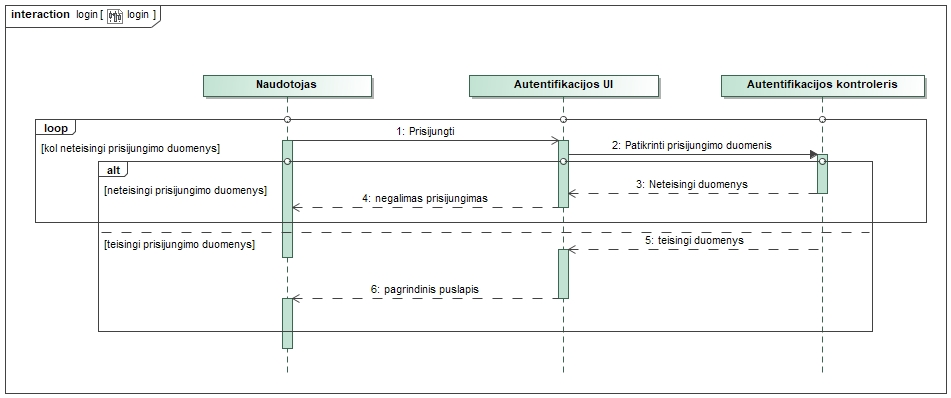
\includegraphics[width=\linewidth]{img/login.jpg}
	\caption{Proceso „Prisijungimas“ sekų diagrama}
	\label{fig:login}
\end{figure}

\subsubsection{Atsijungimas}

\begin{table}[H]
	\caption{Funkciniai reikalavimai. Atsijungimas.}
	\begin{tabular}{|p{1cm}|p{1cm}|p{11,5cm}|p{3,5cm}|}
		\hline 
		\rowcolor{gray!50}
		\multicolumn{2}{|c|}{{\bfseries Kodas}}&
		\multicolumn{1}{c|}{{\bfseries Reikalavimas}}&
		\multicolumn{1}{c|}{{\bfseries Svarba}}\\
		\hline
		\rowcolor{lightgray}
		\multicolumn{4}{|c|}{Atsijungimas}\\		
		
		\hline
		\multicolumn{2}{|c|}{FR 3.1}&
		{Naudotojas paspaudęs mygtuką atsijungti turi būti atjungiamas nuo sistemos.
		}&		
		\multicolumn{1}{c|}{Būtina}\\
		\hline
		\multicolumn{1}{|c}{}&
		\multicolumn{1}{c|}{FR 3.2}&
		{Atsijungus nuo sistemos ir bandant paspausti grįžimo mygtuką naudotojas turi būti nukreipiamas į prisijungimo langą.
		}&		
		\multicolumn{1}{c|}{Būtina}\\
		\hline
	\end{tabular}		
\end{table}

\subsubsection{Paskyros valdymas}

\begin{table}[H]
	\caption{Funkciniai reikalavimai. Paskyros valdymas.}
	\begin{tabular}{|p{1cm}|p{1cm}|p{11,5cm}|p{3,5cm}|}
		\hline 
		\rowcolor{gray!50}
		\multicolumn{2}{|c|}{{\bfseries Kodas}}&
		\multicolumn{1}{c|}{{\bfseries Reikalavimas}}&
		\multicolumn{1}{c|}{{\bfseries Svarba}}\\
		\hline
		\rowcolor{lightgray}
		\multicolumn{4}{|c|}{Paskyros valdymas}\\				
		\hline
		\multicolumn{2}{|c|}{FR 4.1}&
		{Naudotojui paspaudus mygtuką „Mano profilis“ turi būti matoma visa žinoma informacija apie naudotoją.
		}&		
		\multicolumn{1}{c|}{Būtina}\\
		\hline
		\multicolumn{1}{|c}{}&
		\multicolumn{1}{c|}{FR 4.2}&
		{Naudotojui paspaudus mygtuką „Pakeisti slaptažodį“, įvedus tinkamą seną ir naują slaptažodžius bei paspaudus mygtuką „Patvirtinti“ slaptažodis turi būti pakeičiamas į naują.
		}&		
		\multicolumn{1}{c|}{Būtina}\\
		\hline
		\multicolumn{1}{|c}{}&
		\multicolumn{1}{c|}{FR 4.3}&
		{Naudotojui paspaudus mygtuką „Pakeisti slaptažodį“ ir įvedus netinkamą seną slaptažodį turi būti išvedamas klaidos pranešimas.
		}&
		\multicolumn{1}{c|}{Būtina}\\	
		\hline		
		\multicolumn{1}{|c}{}&
		\multicolumn{1}{c|}{FR 4.4}&
		{Naudotojui paspaudus mygtuką „Pakeisti slaptažodį“ ir įvedus netinkamo formato naują slaptažodį turi būti išvedamas klaidos pranešimas ir slaptažodis neturi būti pakeičiamas nauju.
		}&
		\multicolumn{1}{c|}{Būtina}\\									
		\hline
	\end{tabular}		
\end{table}

\subsubsection{Naujienos}

\begin{table}[H]
	\caption{Funkciniai reikalavimai. Naujienos.}
	\begin{tabular}{|p{1cm}|p{1cm}|p{11,5cm}|p{3,5cm}|}
		\hline 
		\rowcolor{gray!50}
		\multicolumn{2}{|c|}{{\bfseries Kodas}}&
		\multicolumn{1}{c|}{{\bfseries Reikalavimas}}&
		\multicolumn{1}{c|}{{\bfseries Svarba}}\\
		\hline
		\rowcolor{lightgray}
		\multicolumn{4}{|c|}{Naujienos}\\		
		
		\hline
		\multicolumn{2}{|c|}{FR 5.1}&
		{Naujienos turi būti matomos pagrindiniame tinklalapio puslapyje.
		}&		
		\multicolumn{1}{c|}{Būtina}\\
		\hline
		\multicolumn{1}{|c}{}&
		\multicolumn{1}{c|}{FR 5.2}&
		{Visas naujienų sąrašas turi būti pateikiamas viename puslapyje.
		}&		
		\multicolumn{1}{c|}{Būtina}\\
		\hline
		\multicolumn{1}{|c}{}&
		\multicolumn{1}{c|}{FR 5.3}&
		{Naujienos turi būti rikiuojamos pagal naujienos paskelbimo datą (naujausios turi būti matomos pirmos).
		}&
		\multicolumn{1}{c|}{Būtina}\\	
		\hline		
		\multicolumn{1}{|c}{}&
		\multicolumn{1}{c|}{FR 5.4}&
		{Jei naujienų sąrašas tuščias turi būti rodomas pranešimas, kad naujienų šiuo metu nėra.
		}&
		\multicolumn{1}{c|}{Būtina}\\									
		\hline
		\multicolumn{1}{|c}{}&
		\multicolumn{1}{c|}{FR 5.5}&
		{Naujienos turi būti matomos visiems prisijungusiems naudotojams.
		}&
		\multicolumn{1}{c|}{Būtina}\\	
		\hline		
		\multicolumn{1}{|c}{}&
		\multicolumn{1}{c|}{FR 5.6}&
		{Naujienos redagavimo funkcija turi būti matoma bei panaudojama tik naujieną paskelbusiam naudotojui.
		}&
		\multicolumn{1}{c|}{Būtina}\\									
		\hline
		\multicolumn{1}{|c}{}&
		\multicolumn{1}{c|}{FR 5.7}&
		{Skelbti naujienas turi būti galimybė tik prisijungusiems dėstytojams bei sistemos administratoriams.
		}&
		\multicolumn{1}{c|}{Būtina}\\	
		\hline		
		\multicolumn{1}{|c}{}&
		\multicolumn{1}{c|}{FR 5.8}&
		{Naujienos ištrynimo funkcija turi būti matoma bei panaudojama tik naujieną paskelbusiam naudotojui bei sistemos administratoriui.
		}&
		\multicolumn{1}{c|}{Būtina}\\									
		\hline
	\end{tabular}		
\end{table}

\ref{fig:delnews} pav. pateikiama užduoties „Naujienos ištrynimas” sekų diagrama. Joje vaizduojamas pagrindinis
naujienos ištrynimo scenarijus.
\begin{figure}[H]
	\centering
	\includegraphics[width=\linewidth]{img/deleteNew.png}
	\caption{Proceso „Naujienos ištrynimas“ sekų diagrama}
	\label{fig:delnews}
\end{figure}

\subsubsection{Renginiai}

\begin{table}[H]
	\caption{Funkciniai reikalavimai. Renginiai.}
	\begin{tabular}{|p{1cm}|p{1cm}|p{11,5cm}|p{3,5cm}|}
		\hline 
		\rowcolor{gray!50}
		\multicolumn{2}{|c|}{{\bfseries Kodas}}&
		\multicolumn{1}{c|}{{\bfseries Reikalavimas}}&
		\multicolumn{1}{c|}{{\bfseries Svarba}}\\
		\hline
		\rowcolor{lightgray}
		\multicolumn{4}{|c|}{Renginiai}\\		
		
		\hline
		\multicolumn{2}{|c|}{FR 6.1}&
		{Renginiai turi būti matomi puslapyje „Renginiai“.
		}&		
		\multicolumn{1}{c|}{Būtina}\\
		\hline
		\multicolumn{1}{|c}{}&
		\multicolumn{1}{c|}{FR 6.2}&
		{Visas renginių sąrašas turi būti pateikiamas kalendoriuje esančiame puslapyje „Renginiai“.
		}&		
		\multicolumn{1}{c|}{Būtina}\\
		\hline
		\multicolumn{1}{|c}{}&
		\multicolumn{1}{c|}{FR 6.3}&
		{Paspaudus ant kalendoriuje pateikto renginio turi atsidaryti puslapis „Renginio informacija“, kuriame renginys turi būti aprašytas detaliau.
		}&
		\multicolumn{1}{c|}{Būtina}\\	
		\hline		
		\multicolumn{1}{|c}{}&
		\multicolumn{1}{c|}{FR 6.4}&
		{Jei nėra sukurta jokių renginiu, puslapyje „Renginiai“ turi būti pateikiamas tuščias kaledorius.
		}&
		\multicolumn{1}{c|}{Būtina}\\									
		\hline
		\multicolumn{1}{|c}{}&
		\multicolumn{1}{c|}{FR 6.5}&
		{Renginiai turi būti matomi visiems prisijungusiems naudotojams.
		}&
		\multicolumn{1}{c|}{Būtina}\\	
		\hline		
		\multicolumn{1}{|c}{}&
		\multicolumn{1}{c|}{FR 6.6}&
		{Renginio redagavimo funkcija turi būti matoma bei panaudojama tik renginį sukūrusiam naudotojui.
		}&
		\multicolumn{1}{c|}{Būtina}\\									
		\hline
		\multicolumn{1}{|c}{}&
		\multicolumn{1}{c|}{FR 6.7}&
		{Kurti renginius turi būti galimybė tik prisijungusiems dėstytojams bei sistemos administratoriams.
		}&
		\multicolumn{1}{c|}{Būtina}\\	
		\hline		
		\multicolumn{1}{|c}{}&
		\multicolumn{1}{c|}{FR 6.8}&
		{Renginio ištrynimo funkcija turi būti matoma bei panaudojama tik naujieną paskelbusiam naudotojui bei sistemos administratoriui.
		}&
		\multicolumn{1}{c|}{Būtina}\\									
		\hline
	\end{tabular}		
\end{table}

\ref{fig:addevent} pav. pateikiama užduoties „Renginio sukūrimas” sekų diagrama. Joje vaizduojamas pagrindinis
renginio sukūrimo scenarijus.
\begin{figure}[H]
	\centering
	\includegraphics[width=\linewidth]{img/addNewEvent.png}
	\caption{Proceso „Renginio sukūrimas“ sekų diagrama}
	\label{fig:addevent}
\end{figure}

\subsubsection{D.U.K.}
\begin{table}[H]
	\caption{Funkciniai reikalavimai. D.U.K.}
	\begin{tabular}{|p{1cm}|p{1cm}|p{11,5cm}|p{3,5cm}|}
		\hline 
		\rowcolor{gray!50}
		\multicolumn{2}{|c|}{{\bfseries Kodas}}&
		\multicolumn{1}{c|}{{\bfseries Reikalavimas}}&
		\multicolumn{1}{c|}{{\bfseries Svarba}}\\
		\hline
		\rowcolor{lightgray}
		\multicolumn{4}{|c|}{D.U.K.}\\		
		
		\hline
		\multicolumn{2}{|c|}{FR 7.1}&
		{Dažniausiai užduodami klausimai turi būti matomi puslapyje „D.U.K.“.
		}&		
		\multicolumn{1}{c|}{Būtina}\\
		\hline
		\multicolumn{1}{|c}{}&
		\multicolumn{1}{c|}{FR 7.2}&
		{Visas dažniausiai užduodamų klausimų sąrašas turi būti pateikiamas viename puslapyje.
		}&		
		\multicolumn{1}{c|}{Būtina}\\
		\hline
		\multicolumn{1}{|c}{}&
		\multicolumn{1}{c|}{FR 7.3}&
		{Paspaudus ant vieno iš pateiktų klausimų turi būti matomas atsakymas į tą klausimą.
		}&
		\multicolumn{1}{c|}{Būtina}\\	
		\hline		
		\multicolumn{1}{|c}{}&
		\multicolumn{1}{c|}{FR 7.4}&
		{D.U.K. turi būti matomi visiems prisijungusiems naudotojams.
		}&
		\multicolumn{1}{c|}{Būtina}\\									
		\hline
		\multicolumn{1}{|c}{}&
		\multicolumn{1}{c|}{FR 7.5}&
		{D.U.K. redagavimo funkcija turi būti matoma bei panaudojama tik sistemos administratoriams.
		}&
		\multicolumn{1}{c|}{Būtina}\\	
		\hline	
		\multicolumn{1}{|c}{}&
		\multicolumn{1}{c|}{FR 7.6}&
		{Sukurti naują klausimą turi būti galimybė tik sistemos administratoriams.
		}&
		\multicolumn{1}{c|}{Būtina}\\	
		\hline	
		\multicolumn{1}{|c}{}&
		\multicolumn{1}{c|}{FR 7.7}&
		{Klausimo ištrynimo funkcija turi būti matoma bei panaudojama tik sistemos administratoriui.
		}&
		\multicolumn{1}{c|}{Būtina}\\	
		\hline	
	\end{tabular}		
\end{table}

\ref{fig:addduk} pav. pateikiama užduoties „D.U.K.pridėjimas” sekų diagrama. Joje vaizduojamas pagrindinis
D.U.K. pridėjimo scenarijus.
\begin{figure}[H]
	\centering
	\includegraphics[width=\linewidth]{img/addDUK.png}
	\caption{Proceso „D.U.K.pridėjimas” sekų diagrama}
	\label{fig:addduk}
\end{figure}

\subsubsection{Dėstytojų sąrašas}

\begin{table}[H]
	\caption{Funkciniai reikalavimai. Dėstytojų sąrašas}
	\begin{tabular}{|p{1cm}|p{1cm}|p{11,5cm}|p{3,5cm}|}
		\hline 
		\rowcolor{gray!50}
		\multicolumn{2}{|c|}{{\bfseries Kodas}}&
		\multicolumn{1}{c|}{{\bfseries Reikalavimas}}&
		\multicolumn{1}{c|}{{\bfseries Svarba}}\\
		\hline
		\rowcolor{lightgray}
		\multicolumn{4}{|c|}{Dėstytojų sąrašas}\\		
		
		\hline
		\multicolumn{2}{|c|}{FR 8.1}&
		{Dėstytojų sąrašas turi būti matomas puslapyje „Dėstytojai“.
		}&		
		\multicolumn{1}{c|}{Būtina}\\
		\hline
		\multicolumn{1}{|c}{}&
		\multicolumn{1}{c|}{FR 8.2}&
		{Puslapyje „Dėstytojai“ turi būti paieškos laukas, kurio pagalba galima surasti reikiamą dėstytoją.
		}&		
		\multicolumn{1}{c|}{Būtina}\\
		\hline
		\multicolumn{1}{|c}{}&
		\multicolumn{1}{c|}{FR 8.3}&
		{Visas dėstytojų sąrašas turi būti pateikiamas viename puslapyje.
		}&
		\multicolumn{1}{c|}{Būtina}\\	
		\hline		
		\multicolumn{1}{|c}{}&
		\multicolumn{1}{c|}{FR 8.4}&
		{Dėstytojai turi būti surikiuoti abecėlės tvarka pagal pavardę ir vardą.
		}&
		\multicolumn{1}{c|}{Būtina}\\									
		\hline
		\multicolumn{1}{|c}{}&
		\multicolumn{1}{c|}{FR 8.5}&
		{Dėstytojų sąrašas turi būti matomas visiems prisijungusiems naudotojams.
		}&
		\multicolumn{1}{c|}{Būtina}\\	
		\hline	
		\multicolumn{1}{|c}{}&
		\multicolumn{1}{c|}{FR 8.6}&
		{Prie dėstytojo vardo bei pavardės turi būti pateikiamos nuorodos į dėstytojo puslapį bei į žinutės išsiuntimo dėstytojui puslapį.
		}&
		\multicolumn{1}{c|}{Būtina}\\	
		\hline		
	\end{tabular}		
\end{table}

\subsubsection{Dėstytojo puslapis}

\begin{table}[H]
	\caption{Funkciniai reikalavimai. Dėstytojo puslapis}
	\begin{tabular}{|p{1cm}|p{1cm}|p{11,5cm}|p{3,5cm}|}
		\hline 
		\rowcolor{gray!50}
		\multicolumn{2}{|c|}{{\bfseries Kodas}}&
		\multicolumn{1}{c|}{{\bfseries Reikalavimas}}&
		\multicolumn{1}{c|}{{\bfseries Svarba}}\\
		\hline
		\rowcolor{lightgray}
		\multicolumn{4}{|c|}{Dėstytojo puslapis}\\		
		
		\hline
		\multicolumn{2}{|c|}{FR 9.1}&
		{Dėstytojo puslapis turi būti matomas visiems prisijungusiems naudotojams.
		}&		
		\multicolumn{1}{c|}{Būtina}\\
		\hline
		\multicolumn{1}{|c}{}&
		\multicolumn{1}{c|}{FR 9.2}&
		{Tik prisijungęs dėstytojas turi galimybę sukurti savo puslapį.
		}&		
		\multicolumn{1}{c|}{Būtina}\\
		\hline
		\multicolumn{1}{|c}{}&
		\multicolumn{1}{c|}{FR 9.3}&
		{Tik prisijungęs dėstytojas sukūręs savo puslapį turi galimybę jį redaguoti.
		}&
		\multicolumn{1}{c|}{Būtina}\\	
		\hline		
		\multicolumn{1}{|c}{}&
		\multicolumn{1}{c|}{FR 9.4}&
		{Dėstytojo puslapyje turi buti nuoroda, kurią paspaudus turi būti galimybė rašyti žinutę pasirinktam dėstytojui.
		}&
		\multicolumn{1}{c|}{Būtina}\\									
		\hline
	\end{tabular}		
\end{table}

\ref{fig:editpage} pav. pateikiama užduoties „Dėstytojo puslapio redagavimas” sekų diagrama. Joje vaizduojamas pagrindinis dėstytojo puslapio redagavimo scenarijus.
\begin{figure}[H]
	\centering
	\includegraphics[width=\linewidth]{img/editPage.png}
	\caption{Proceso „Dėstytojo puslapio redagavimas” sekų diagrama}
	\label{fig:editpage}
\end{figure}

\subsubsection{Žinutės}

\begin{table}[H]
	\caption{Funkciniai reikalavimai. Žinutės}
	\begin{tabular}{|p{1cm}|p{1cm}|p{11,5cm}|p{3,5cm}|}
		\hline 
		\rowcolor{gray!50}
		\multicolumn{2}{|c|}{{\bfseries Kodas}}&
		\multicolumn{1}{c|}{{\bfseries Reikalavimas}}&
		\multicolumn{1}{c|}{{\bfseries Svarba}}\\
		\hline
		\rowcolor{lightgray}
		\multicolumn{4}{|c|}{Žinutės}\\		
		
		\hline
		\multicolumn{2}{|c|}{FR 10.1}&
		{Puslapis „Žinutės“ turi būti matomas visiems prisijungusiems naudotojams.
		}&		
		\multicolumn{1}{c|}{Būtina}\\
		\hline
		\multicolumn{1}{|c}{}&
		\multicolumn{1}{c|}{FR 10.2}&
		{Puslapyje „Žinutės“ turi būti pateikiamos visos gautos bei išsiųstos žinutės.
		}&		
		\multicolumn{1}{c|}{Būtina}\\
		\hline
		\multicolumn{1}{|c}{}&
		\multicolumn{1}{c|}{FR 10.3}&
		{Visoms gautoms bei išsiųstoms žinutėms pateikti naudojami puslapiai (viename puslapyje 25 žinutės).
		}&
		\multicolumn{1}{c|}{Būtina}\\	
		\hline		
		\multicolumn{1}{|c}{}&
		\multicolumn{1}{c|}{FR 10.4}&
		{Išsiųsti žinutę turi turėti galimybę visi prisijungę naudotojai.
		}&
		\multicolumn{1}{c|}{Būtina}\\									
		\hline
		\multicolumn{1}{|c}{}&
		\multicolumn{1}{c|}{FR 10.5}&
		{Dėstytojo puslapyje turi buti nuoroda, kurią paspaudus galima būtų rašyti žinutę pasirinktam dėstytojui.
		}&
		\multicolumn{1}{c|}{Būtina}\\	
		\hline	
		\multicolumn{1}{|c}{}&
		\multicolumn{1}{c|}{FR 10.6}&
		{Paspaudus mygtuką „Išsiųsti žinutę“ turi atsidaryti žinutės rašymo langas, kuriame turi būti galimybė pasirinkti naudotoją, kuriam žinutė bus išsiųsta.
		}&
		\multicolumn{1}{c|}{Būtina}\\	
		\hline		
		\multicolumn{1}{|c}{}&
		\multicolumn{1}{c|}{FR 10.7}&
		{Paspaudus žinutės išsiuntimo patvirtinimo mygtuką, žinutė turi būti nusiųstą naudotojui, kuriam ši žinutė turėjo būti išsiųsta.
		}&
		\multicolumn{1}{c|}{Būtina}\\									
		\hline
		\multicolumn{1}{|c}{}&
		\multicolumn{1}{c|}{FR 10.8}&
		{Turi būti galimybė išsiųsti žinutę daugiau nei vienam naudotojui vienu metu.
		}&
		\multicolumn{1}{c|}{Būtina}\\	
		\hline	
		\multicolumn{1}{|c}{}&
		\multicolumn{1}{c|}{FR 10.9}&
		{Dėstytojas turi turėti galimybę pasirinkti išsiųsti žinutę visai grupei arba kursui studentų.
		}&
		\multicolumn{1}{c|}{Būtina}\\	
		\hline		
	\end{tabular}		
\end{table}

\ref{fig:sendmessage} pav. pateikiama užduoties „Žinutės išsiuntimas” sekų diagrama. Joje vaizduojamas pagrindinis žinutės išsiuntimo scenarijus.
\begin{figure}[H]
	\centering
	\includegraphics[width=\linewidth]{img/sendMes.png}
	\caption{Proceso „Žinutės išsiuntimas” sekų diagrama}
	\label{fig:sendmessage}
\end{figure}

\subsubsection{Konspektai}

\begin{table}[H]
	\caption{Funkciniai reikalavimai. Konspektai}
	\begin{tabular}{|p{1cm}|p{1cm}|p{11,5cm}|p{3,5cm}|}
		\hline 
		\rowcolor{gray!50}
		\multicolumn{2}{|c|}{{\bfseries Kodas}}&
		\multicolumn{1}{c|}{{\bfseries Reikalavimas}}&
		\multicolumn{1}{c|}{{\bfseries Svarba}}\\
		\hline
		\rowcolor{lightgray}
		\multicolumn{4}{|c|}{Konspektai}\\		
		
		\hline
		\multicolumn{2}{|c|}{FR 11.1}&
		{Puslapis „Konspektai“ turi būti matomas visiems prisijungusiems studentams bei sistemos administratoriui.
		}&		
		\multicolumn{1}{c|}{Būtina}\\
		\hline
		\multicolumn{1}{|c}{}&
		\multicolumn{1}{c|}{FR 11.2}&
		{Konspektai turi būti pateikiami šalia dėstomo dalyko pavadinimo, o dėstomi dalykai turi būti surikiuoti abecėlės tvarka.
		}&		
		\multicolumn{1}{c|}{Būtina}\\
		\hline
		\multicolumn{1}{|c}{}&
		\multicolumn{1}{c|}{FR 11.3}&
		{Puslapyje „Konspektai“ turi būti paieškos laukelis, kuriame turi būti galimybė ieškoti dėstomo dalyko.
		}&
		\multicolumn{1}{c|}{Būtina}\\	
		\hline		
		\multicolumn{1}{|c}{}&
		\multicolumn{1}{c|}{FR 11.4}&
		{Puslapyje „Konspektai“ turi būti pateikiami visi studentų įkelti konspektai.
		}&
		\multicolumn{1}{c|}{Būtina}\\									
		\hline
		\multicolumn{1}{|c}{}&
		\multicolumn{1}{c|}{FR 11.5}&
		{Įkelti konspektą turi turėti galimybę visi prisijungę studentai.
		}&
		\multicolumn{1}{c|}{Būtina}\\	
		\hline	
		\multicolumn{1}{|c}{}&
		\multicolumn{1}{c|}{FR 11.6}&
		{Paspaudus mygtuką „Įkelti konspektą“ turi atsidaryti failų pasirinkimo langas.
		}&
		\multicolumn{1}{c|}{Būtina}\\	
		\hline		
		\multicolumn{1}{|c}{}&
		\multicolumn{1}{c|}{FR 11.7}&
		{Paspaudus konspekto įkėlimo patvirtinimo mygtuką, konspektas turi atsirasti visų konspektų sąraše.
		}&
		\multicolumn{1}{c|}{Būtina}\\									
		\hline
		\multicolumn{1}{|c}{}&
		\multicolumn{1}{c|}{FR 11.8}&
		{Įkeliant konspektą turi būti nurodomas dėstomas dalykas.
		}&
		\multicolumn{1}{c|}{Būtina}\\	
		\hline		
	\end{tabular}		
\end{table}

\ref{fig:summary} pav. pateikiama užduoties „Konspekto įkėlimas” sekų diagrama. Joje vaizduojamas pagrindinis konpekto įkėlimo scenarijus ir taip pat nagrinėjami alternatyvūs scenarijai.
\begin{figure}[H]
	\centering
	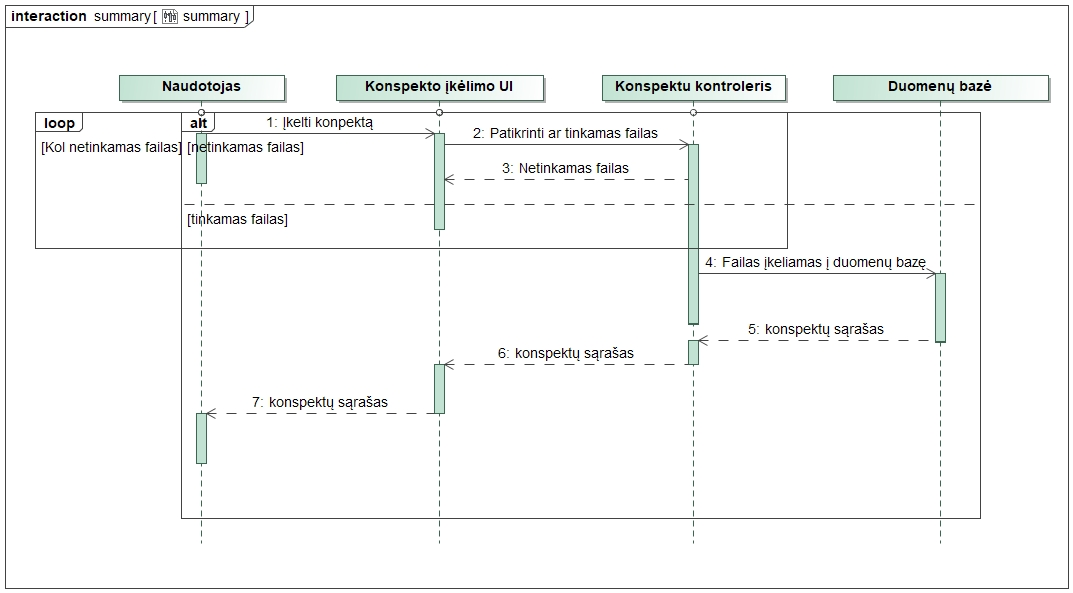
\includegraphics[width=\linewidth]{img/summary.jpg}
	\caption{Proceso „Konspekto įkėlimas“ sekų diagrama}
	\label{fig:summary}
\end{figure}
\newpage

\subsection{NEFUNKCINIAI REIKALAVIMAI}
2-ame skyriuje pateikiami nefunkciniai reikalavimai bei jų svarba. Aprašoma, kaip sistema turi veikti ir kaip ji turi būti kuriama.
\subsubsection{Vidinių interfeisų reikalavimai}
\begin{table}[H]
	\caption{Nefunkciniai reikalavimai. Vidinių interfeisų reikalavimai.}
	\begin{tabular}{|p{1cm}|p{1cm}|p{11,5cm}|p{3,5cm}|}
		\hline 
		\rowcolor{gray!50}
		\multicolumn{2}{|c|}{{\bfseries Kodas}}&
		\multicolumn{1}{c|}{{\bfseries Reikalavimas}}&
		\multicolumn{1}{c|}{{\bfseries Svarba}}\\
		\hline
		\rowcolor{lightgray}
		\multicolumn{4}{|c|}{Vidinių interfeisų reikalavimai}\\		
		
		\hline
		\multicolumn{4}{|c|}{\bfseries OS naudojimo reikalavimai}\\	
		
		\hline
		\multicolumn{2}{|c|}{NFR 1.1}&
		{Tinklapis pritaikytas tiek kompiuteriams, tiek mobiliesiems įrenginiams.
		}&		
		\multicolumn{1}{c|}{Būtina}\\
		\hline
		\multicolumn{1}{|c}{}&
		\multicolumn{1}{c|}{NFR 1.2}&
		{Puslapis pasiekiamas per visas populiariausias naršykles
			(Google Chrome, Mozilla Firefox, IE (nuo 8 versijos), Edge, Safari).
		}&		
		\multicolumn{1}{c|}{Būtina}\\
		
		\hline
		\multicolumn{4}{|c|}{\bfseries Sąveikos su DB reikalavimai}\\		
		
		\hline
		\multicolumn{1}{|c}{}&
		\multicolumn{1}{c|}{NFR 2.1}&
		{Tinklapis turi turėti duomenų bazę, kurioje saugomi naudotojų duomenys, renginiai, D.U.K., konspektai bei dėstytojų puslapių informacija.
		}&
		\multicolumn{1}{c|}{Būtina}\\	
		\hline		
		\multicolumn{1}{|c}{}&
		\multicolumn{1}{c|}{NFR 2.2}&
		{Duomenys saugomi reliaciniu būdu, naudojama MySQL
			duomenų bazių valdymo sistema.
		}&
		\multicolumn{1}{c|}{Būtina}\\		
		
		\hline		
		\multicolumn{1}{|c}{}&
		\multicolumn{1}{c|}{NFR 2.3}&
		{Naudojama Microsoft Azure SQL Database paslauga.
		}&
		\multicolumn{1}{c|}{Pageidautina}\\	
		
		
		\hline
		\multicolumn{4}{|c|}{\bfseries Dokumentų mainų reikalavimai}\\		
		
		\hline
		\multicolumn{2}{|c|}{NFR 3.1}&
		{Naudotojų įkeliamos nuotraukos turi būti,.jpg, .png, .bmp formato bei neviršyti 5MB dydžio.
		}&
		\multicolumn{1}{c|}{Būtina}\\
		
		\hline
		\multicolumn{4}{|c|}{\bfseries Darbo kompiuterių tinkluose reikalavimai}\\		
		
		\hline
		\multicolumn{1}{|c}{}&
		\multicolumn{1}{c|}{NFR 4.1}&
		{Duomenys perduodami naudojant HTTPS protokolą.
		}&
		\multicolumn{1}{c|}{Būtina}\\	
		
		\hline
		\multicolumn{4}{|c|}{\bfseries Sąveikos su kitomis programomis reikalavimai}\\	
		\hline
		\multicolumn{1}{|c}{}&
		\multicolumn{1}{c|}{NFR 5.1}&
		{Vartotojo autentifikacija vykdoma per is.vu.lt sistemą.
		}&
		\multicolumn{1}{c|}{Būtina}\\
		
		\hline
		\multicolumn{4}{|c|}{\bfseries Programavimo aplinkos reikalavimai}\\	
		\hline
		\multicolumn{1}{|c}{}&
		\multicolumn{1}{c|}{NFR 6.1}&
		{Tinklapis kuriamas PHP programavimo kalba, naudojant
			Symfony karkasą.
		}&
		\multicolumn{1}{c|}{Būtina}\\		
		
		\hline
		\multicolumn{1}{|c}{}&
		\multicolumn{1}{c|}{NFR 6.2}&
		{Kodo saugojimui ir dalinimuisi naudojama privati Github repositorija.
		}&
		\multicolumn{1}{c|}{Pageidautina}\\	
		
		\hline
		\multicolumn{1}{|c}{}&
		\multicolumn{1}{c|}{NFR 6.3}&
		{Naudojama PHPStorm programavimo aplinka.
		}&
		\multicolumn{1}{c|}{Pageidautina}\\									
		
		\hline
	\end{tabular}		
\end{table}


\subsubsection{Veikimo reikalavimai}
\begin{table}[H]
	\caption{Nefunkciniai reikalavimai. Veikimo reikalavimai.}
	\begin{tabular}{|p{1cm}|p{1cm}|p{11,5cm}|p{3,5cm}|}
		\hline 
		\rowcolor{gray!50}
		\multicolumn{2}{|c|}{{\bfseries Kodas}}&
		\multicolumn{1}{c|}{{\bfseries Reikalavimas}}&
		\multicolumn{1}{c|}{{\bfseries Svarba}}\\
		\hline
		\rowcolor{lightgray}
		\multicolumn{4}{|c|}{Veikimo reikalavimai}\\		
		
		\hline
		\multicolumn{4}{|c|}{\bfseries Vaizdavimo reikalavimai}\\	
		
		\hline
		\multicolumn{2}{|c|}{NFR 7.1}&
		{Tinklapis turi būti palaikomas visose populiariausiose naršyklėse (IE (nuo 8 versijos), Edge, Chrome, Safari, Firefox).
		}&		
		\multicolumn{1}{c|}{Būtina}\\
		\hline
		\multicolumn{1}{|c}{}&
		\multicolumn{1}{c|}{NFR 7.2}&
		{Keičiant naršyklės dydį, tinklapis vaizdą pritaiko automatiškai.).
		}&		
		\multicolumn{1}{c|}{Būtina}\\
		
		\hline
		\multicolumn{1}{|c}{}&
		\multicolumn{1}{c|}{NFR 7.3}&
		{Data turi būti vaizduojama formatu YYYY-MM-DD, kur
			YYYY – metai, MM – mėnuo, DD – diena.
		}&		
		\multicolumn{1}{c|}{Būtina}\\
		
		\hline
		\multicolumn{1}{|c}{}&
		\multicolumn{1}{c|}{NFR 7.4}&
		{Laikas turi būti vaizduojamas formatu hh:mm, kur hh - valandos, mm - minutės.
		}&		
		\multicolumn{1}{c|}{Būtina}\\
		
		\hline
		\multicolumn{1}{|c}{}&
		\multicolumn{1}{c|}{NFR 7.5}&
		{Pavadinimai – ne daugiau 50 simbolių.
		}&		
		\multicolumn{1}{c|}{Būtina}\\
		
		\hline
		\multicolumn{4}{|c|}{\bfseries Robastiškumo reikalavimai}\\		
		
		\hline
		\multicolumn{1}{|c}{}&
		\multicolumn{1}{c|}{NFR 8.1}&
		{Sistemoje turi būti įdiegtos apsaugos priemonės nuo duomenų sugadinimo, praradimo, klaidingų duomenų įvedimo į DB.
		}&
		\multicolumn{1}{c|}{Būtina}\\	
		\hline		
		\multicolumn{1}{|c}{}&
		\multicolumn{1}{c|}{NFR 8.2}&
		{Pranešti naudotojui, jei interneto ryšys nutrūko.
		}&
		\multicolumn{1}{c|}{Pageidautina}\\		
		
		\hline
		\multicolumn{4}{|c|}{\bfseries Našumo reikalavimai}\\		
		
		\hline
		\multicolumn{2}{|c|}{NFR 9.1}&
		{Užklausai įvykdyti turi užtekti ne daugiau nei 5 sekundžių.
		}&
		\multicolumn{1}{c|}{Būtina}\\
		
		\hline
		\multicolumn{4}{|c|}{\bfseries Darbo kompiuterių tinkluose reikalavimai}\\		
		
		\hline
		\multicolumn{1}{|c}{}&
		\multicolumn{1}{c|}{NFR 10.1}&
		{Svetainės talpinimo (hostingo) planas turi būti parinktas atsižvelgiant į prognozuojamą klientų srautą. Rekomenduojamas duomenų srautas – 50GB/mėn., vieta serveryje - iki 3GB.
		}&
		\multicolumn{1}{c|}{Būtina}\\
		
		\hline
		\multicolumn{1}{|c}{}&
		\multicolumn{1}{c|}{NFR 10.1}&
		{Didžiausia leistina tinklapio sistemos apkrova yra 1000 naudotojų, prisijungusių vienu metu.
		}&
		\multicolumn{1}{c|}{Būtina}\\
		\hline
	\end{tabular}		
\end{table}
\subsubsection{Diegimo reikalavimai}
\begin{table}[H]
	\caption{Nefunkciniai reikalavimai. Diegimo reikalavimai.}
	\begin{tabular}{|p{1cm}|p{1cm}|p{11,5cm}|p{3,5cm}|}
		\hline 
		\rowcolor{gray!50}
		\multicolumn{2}{|c|}{{\bfseries Kodas}}&
		\multicolumn{1}{c|}{{\bfseries Reikalavimas}}&
		\multicolumn{1}{c|}{{\bfseries Svarba}}\\
		\hline
		\rowcolor{lightgray}
		\multicolumn{4}{|c|}{Diegimo reikalavimai}\\		
		
		\hline
		\multicolumn{4}{|c|}{\bfseries Ruošinio reikalavimai}\\	
		
		\hline
		\multicolumn{2}{|c|}{NFR 11.1}&
		{Dokumentacija
		}&		
		\multicolumn{1}{c|}{Būtina}\\
		\hline
		\multicolumn{1}{|c}{}&
		\multicolumn{1}{c|}{NFR 11.2}&
		{Hostingo prisijungimo duomenys.
		}&		
		\multicolumn{1}{c|}{Būtina}\\
		
		\hline
		\multicolumn{1}{|c}{}&
		\multicolumn{1}{c|}{NFR 11.3}&
		{MS Azure prisijungimo duomenys.
		}&		
		\multicolumn{1}{c|}{Pageidautina}\\
		
		
		\hline
		\multicolumn{4}{|c|}{\bfseries Instaliavimo reikalavimai}\\		
		
		\hline
		\multicolumn{1}{|c}{}&
		\multicolumn{1}{c|}{NFR 12.1}&
		{Apsilankęs internetiniame pusalpyje, vartotojas privalo sutikti su slapukų naudojimo sąlygomis.
		}&
		\multicolumn{1}{c|}{Būtina}\\	
		
		\hline
		\multicolumn{4}{|c|}{\bfseries Pradinio DB kaupimo reikalavimai}\\		
		
		\hline
		\multicolumn{2}{|c|}{NFR 13.1}&
		{Turi būti sukurtos lentelės.}&
		\multicolumn{1}{c|}{Būtina}\\
		
		\hline
		\multicolumn{2}{|c|}{NFR 13.2}&
		{Naudotojų lentelėje turi būti administratoriaus duomenys.}&
		\multicolumn{1}{c|}{Būtina}\\	
		
		\hline
		\multicolumn{4}{|c|}{\bfseries Sistemos įsisavinamumo reikalavimai}\\		
		
		\hline
		\multicolumn{1}{|c}{}&
		\multicolumn{1}{c|}{NFR 14.1}&
		{Sistema turi funkcionuoti dvejomis kalbomis: lietuvių ir anglų.}&
		\multicolumn{1}{c|}{Būtina}\\
		
		\hline
		\multicolumn{1}{|c}{}&
		\multicolumn{1}{c|}{NFR 14.2}&
		{Negali būti klaidinančių nuorodų.}&
		\multicolumn{1}{c|}{Būtina}\\
		
		\hline
		\multicolumn{1}{|c}{}&
		\multicolumn{1}{c|}{NFR 14.3}&
		{Ikonos turi atspindėti mygtuko panaudojimą.}&
		\multicolumn{1}{c|}{Būtina}\\
		
		\hline
	\end{tabular}		
\end{table}
\subsubsection{Aptarnavimo ir priežiūros reikalavimai}
\begin{table}[H]
	\caption{Nefunkciniai reikalavimai. Aptarnavimo ir priežiūros reikalavimai.}
	\begin{tabular}{|p{1cm}|p{1cm}|p{11,5cm}|p{3,5cm}|}
		\hline 
		\rowcolor{gray!50}
		\multicolumn{2}{|c|}{{\bfseries Kodas}}&
		\multicolumn{1}{c|}{{\bfseries Reikalavimas}}&
		\multicolumn{1}{c|}{{\bfseries Svarba}}\\
		\hline
		\rowcolor{lightgray}
		\multicolumn{4}{|c|}{Aptarnavimo ir priežiūros reikalavimai}\\		
		
		\hline
		\multicolumn{2}{|c|}{NFR 15.1}&
		{Atsiradęs naujas funkcionalumas turi būti įdiegtas per 5 darbo dienas.
		}&		
		\multicolumn{1}{c|}{Būtina}\\
		\hline
		\multicolumn{1}{|c}{}&
		\multicolumn{1}{c|}{NFR 15.2}&
		{Rasta klaida turi būti ištaisyta per 2 darbo dienas.
		}&		
		\multicolumn{1}{c|}{Būtina}\\
		
		\hline
		\multicolumn{1}{|c}{}&
		\multicolumn{1}{c|}{NFR 15.3}&
		{Į naudotojo laiškus su pastebėjimais ir skundais atsakyti reikia per 3 darbo dienas.
		}&		
		\multicolumn{1}{c|}{Pageidautina}\\
		
		\hline
		\multicolumn{1}{|c}{}&
		\multicolumn{1}{c|}{NFR 15.4}&
		{Jei dėl planuojamo atnaujinimo reikės trumpam sustabdyti
			sistemos veiklą, naudotojai turi būti iš anksto įspėti ne mažiau nei prieš 24 val.
		}&		
		\multicolumn{1}{c|}{Pageidautina}\\	
		
		\hline
	\end{tabular}		
\end{table}
\subsubsection{Tiražuojamumo reikalavimai}
\begin{table}[H]
	\caption{Nefunkciniai reikalavimai. Tiražuojamumo reikalavimai.}
	\begin{tabular}{|p{1cm}|p{1cm}|p{12,5cm}|p{3,5cm}|}
		\hline 
		\rowcolor{gray!50}
		\multicolumn{2}{|c|}{{\bfseries Kodas}}&
		\multicolumn{1}{c|}{{\bfseries Reikalavimas}}&
		\multicolumn{1}{c|}{{\bfseries Svarba}}\\
		\hline
		\rowcolor{lightgray}
		\multicolumn{4}{|c|}{Tiražuojamumo reikalavimai}\\		
		
		\hline
		\multicolumn{2}{|c|}{NFR 16.1}&
		{Internetinė svetainė turi veikti bet kuriame įrenginyje, kuris turi naršyklę ir interneto ryšį.
		}&		
		\multicolumn{1}{c|}{Būtina}\\
		
		\hline
	\end{tabular}		
\end{table}
\subsubsection{Apsaugos reikalavimai}
\begin{table}[H]
	\caption{Nefunkciniai reikalavimai. Apsaugos reikalavimai.}
	\begin{tabular}{|p{1cm}|p{1cm}|p{12,5cm}|p{3,5cm}|}
		\hline 
		\rowcolor{gray!50}
		\multicolumn{2}{|c|}{{\bfseries Kodas}}&
		\multicolumn{1}{c|}{{\bfseries Reikalavimas}}&
		\multicolumn{1}{c|}{{\bfseries Svarba}}\\
		\hline
		\rowcolor{lightgray}
		\multicolumn{4}{|c|}{Apsaugos reikalavimai}\\		
		
		\hline
		\multicolumn{2}{|c|}{NFR 17.1}&
		{Naudotojui prisijungiant prie sistemos vykdoma jo identifikacija.
		}&		
		\multicolumn{1}{c|}{Būtina}\\
		
		\hline
		\multicolumn{2}{|c|}{NFR 17.2}&
		{Atsarginės DB kopijos daromos ne rečiau nei kas savaitę.
		}&		
		\multicolumn{1}{c|}{Būtina}\\	
		
		\hline
		\multicolumn{2}{|c|}{NFR 17.3}&
		{Jei naudotojas neaktyvus ilgiau nei 30 minučių, jis turi būti automatiškai atjungiamas nuo sistemos.
		}&		
		\multicolumn{1}{c|}{Būtina}\\		
		
		\hline
	\end{tabular}		
\end{table}
\subsubsection{Juridiniai reikalavimai}
\begin{table}[H]
	\caption{Nefunkciniai reikalavimai. Juridiniai reikalavimai.}
	\begin{tabular}{|p{1cm}|p{1cm}|p{12,5cm}|p{3,5cm}|}
		\hline 
		\rowcolor{gray!50}
		\multicolumn{2}{|c|}{{\bfseries Kodas}}&
		\multicolumn{1}{c|}{{\bfseries Reikalavimas}}&
		\multicolumn{1}{c|}{{\bfseries Svarba}}\\
		\hline
		\rowcolor{lightgray}
		\multicolumn{4}{|c|}{Juridiniai reikalavimai}\\		
		
		\hline
		\multicolumn{2}{|c|}{NFR 18.1}&
		{Kuriant sistemą projekto komanda neturi naudotis nelegalia
			programine įranga.
		}&		
		\multicolumn{1}{c|}{Būtina}\\
		
		\hline
		\multicolumn{2}{|c|}{NFR 18.2}&
		{Internetinėje svetainėje turi būti galimybė peržiūrėti naudojimosi sąlygas.
		}&		
		\multicolumn{1}{c|}{Būtina}\\				
		\hline
	\end{tabular}		
\end{table}
\newpage

\subsection{VARTOTOJO SĄSAJOS REIKALAVIMAI}
3 skyriuje pateikiami vartotojo sąsajos reikalavimai, kuriuose pateikiama informaciją apie sistemos grafinį vaizdą, kurį mato vartotojas. Nagrinėjami naudotojui matomi puslapiai, ikonos, simboliai bei mygtukai, pavaizduoti prototipuose (žr. 1 priedas). Taip pat aprašomos jų funkcijos, paskirtys bei svarbumas.

\subsubsection{Dalykinės srities metaforos reikalavimai}
\begin{table}[H]
	\caption{Vartotojo interfeiso reikalavimai. Dalykinės srities metaforos reikalavimai.}
	\begin{tabular}{|p{1cm}|p{1cm}|p{12,5cm}|p{3,5cm}|}
		\hline
		\rowcolor{lightgray}
		\multicolumn{4}{|c|}{1. Dalykinės srities metaforos reikalavimai}\\		
		\hline 
		\rowcolor{gray!50}
		\multicolumn{2}{|c|}{{\bfseries Kodas}}&
		\multicolumn{1}{c|}{{\bfseries Reikalavimas}}&
		\multicolumn{1}{c|}{{\bfseries Svarba}}\\
		\hline
		\multicolumn{2}{|c|}{VIR 1.1}&
		{Pagrindinio puslapio atidarymas arba perkrovimas yra vaizduojamas puslapio logotipu}&		
		\multicolumn{1}{c|}{Būtinas}\\
		\hline
		\multicolumn{2}{|c|}{VIR 1.2}&
		{Renginio arba naujienos įkėlimas yra vaizduojamas pliuso simboliu.}&		
		\multicolumn{1}{c|}{Pageidautina}\\	
		\hline
		\multicolumn{2}{|c|}{VIR 1.3}&
		{Renginio arba naujienos redagavimas yra vaizduojamas pieštuko simboliu.}&		
		\multicolumn{1}{c|}{Pageidautina}\\	
		\hline
		\multicolumn{2}{|c|}{VIR 1.4}&
		{Renginiai išdėstyti nuo eilės tvarka nuo artimiausios datos iki tolimiausios}&		
		\multicolumn{1}{c|}{Būtina}\\				
		\hline
	\end{tabular}		
\end{table}


\begin{longtable}{|p{2cm}|p{11,5cm}|p{2cm}|}\toprule
	\caption{Vartotojo interfeiso reikalavimai. Užduočių reikalavimai}\\
	\hline  \rowcolor{lightgray} 
	\multicolumn{3}{|c|}{2. Užduočių reikalavimai}\\ \hline 
	\multicolumn{1}{|l|}{\textbf{Kodas}} & \multicolumn{1}{c|}{\textbf{Reikalavimas}} & \multicolumn{1}{c|}{\textbf{Svarba}} \\ \hline 
	\multicolumn{3}{|c|}{Neprisiregistravusio naudotojo sąsajos užduotys}\\ \hline
	{VIR3.1}&{Prisiregistruoti prie aplikacijos}&{Būtinas} \\ \hline
	{VIR2.2}&{Susipažinti su puslapio taisyklėmis}&{Būtinas}\\ \hline
	\multicolumn{3}{|c|}{Dėstytojo sąsajos užduotys}\\ \hline
	{VIR3.1}&{Prisijungti prie savo paskyros}&{Būtinas}\\ \hline
	{VIR3.2}&{Redaguoti savo prisijungimo slaptažodį}&{Būtinas}\\ \hline
	{VIR3.3}&{Atsijungti iš savo paskyros}&{Būtinas}\\ \hline
	{VIR3.4}&{Pridėti naujieną}&{Būtinas}\\ 	\hline
	{VIR3.5}&{Redaguoti renginį}&{Būtinas}\\	\hline
	{VIR3.6}&{Ištrinti renginį}&{Būtinas}\\ 	\hline
	{VIR3.7}&{Pridėti renginį}&{Būtinas}\\ 	\hline
	{VIR3.8}&{Redaguoti renginį}&{Būtinas}\\ 	\hline
	{VIR3.9}&{Ištrinti renginį}&{Būtinas}\\	\hline
	{VIR3.10}&{Siųsti žinutę}&{Būtinas}\\ 	\hline
	{VIR3.11}&{Peržiūrėti visas žinutes}&{Būtinas}\\ 	\hline
	{VIR3.12}&{Gauti žinutes}&{Būtinas}\\ 	\hline
	{VIR3.13}&{Peržvelgti visas naujienas}&{Būtinas}\\	\hline
	{VIR3.14}&{Peržvelgti visus renginius}&{Būtinas}\\	\hline
	{VIR3.15}&{Peržiūrėti D.U.K.}&{Būtinas}\\	\hline
	{VIR3.16}&{Pridėti D.U.K.}&{Būtinas}\\ 	\hline
	{VIR3.17}&{Peržiūrėti D.U.K.}&{Būtinas}\\	\hline
	{VIR3.18}&{Peržvelgti visus dėstytojus}&{Būtinas}\\ 	\hline
	{VIR3.19}&{Redaguoti asmeninį tinklalapį}&{Būtinas}\\ 	\hline
	\multicolumn{3}{|c|}{Studento sąsajos užduotys}\\	\hline
	{VIR4.1}&{Prisijungti prie savo paskyros}&{Būtinas}\\	\hline
	{VIR4.2}&{Redaguoti savo prisijungimo slaptažodį}&{Būtinas}\\	\hline
	{VIR4.3}&{Atsijungti iš savo paskyros}&{Būtinas}\\	\hline
	{VIR4.4}&{Siųsti žinutę}&{Būtinas}\\	\hline
	{VIR4.5}&{Peržiūrėti visas žinutes}&{Būtinas}\\	\hline
	{VIR4.6}&{Gauti žinutes}&{Būtinas}\\	\hline
	{VIR4.7}&{Peržvelgti visas naujienas}&{Būtinas}\\	\hline
	{VIR4.8}&{Peržvelgti visus renginius}&{Būtinas}\\	\hline
	{VIR4.9}&{Peržiūrėti D.U.K.}&{Būtinas}\\	\hline
	{VIR4.10}&{Peržiūrėti D.U.K.}&{Būtinas}\\	\hline
	{VIR4.11}&{Peržvelgti visus dėstytojus}&{Būtinas}\\	\hline
	{VIR4.12}&{Peržiūrėti konkretaus dėstytojo puslapį ir informaciją jame}&{Būtinas}\\	\hline
	{VIR4.13}&{Peržiūrėti visus konspektus}&{Būtinas}\\	\hline
	{VIR4.14}&{Įkelti konspektą}&{Būtinas}\\	\hline
	\multicolumn{3}{|c|}{Administratoriaus sąsajos reikalavimai}\\	\hline
	{VIR5.1}&{Pridėti naujienas/renginius/D.U.K.}&{Būtinas}\\	\hline
	{VIR5.2}&{Peržiūrėti naujienas/renginius/D.U.K. ir pašalinti nebeaktualius}&{Būtinas}\\	\hline
	{VIR5.3}&{Kurti sąrašus duomenų bazėje}&{Būtinas}\\	\hline
	{VIR5.4}&{Atnaujinti tinklalapį}&{Būtinas}\\	\hline
	{VIR5.5}&{Patikrinti konspektų turinį}&{Būtinas}\\	\hline
	{VIR5.6}&{Taisyti tinklalapio klaidas}&{Būtinas}\\	\hline
	{VIR5.7}&{Blokuoti naudotojus}&{Būtinas}\\	\hline
	\multicolumn{3}{|c|}{Bendri reikalavimai}\\	\hline
	{VIR6.1}&{Puslapio viršuje visada esantis meniu}&{Būtinas}\\	\hline
	{VIR6.2}&{Teksto įvedimo formų laukai}&{Būtinas}\\	\hline
	{VIR6.3}&{Ikonos}&{Būtinas}\\	\hline
	{VIR6.4}&{Matomas atsijungimo mygtukas}&{Būtinas}\\	\hline
\end{longtable}

\subsubsection{Užduočių formulavimo kalbos reikalavimai}
\begin{table}[H]
	\caption{Vartotojo interfeiso reikalavimai. Užduočių formulavimo kalbos reikalavimai}
	\begin{tabular}{|p{1cm}|p{1cm}|p{11,5cm}|p{3,5cm}|}
		\hline
		\rowcolor{lightgray}
		\multicolumn{4}{|c|}{3. Užduočių formulavimo kalbos reikalavimai}\\		
		\hline 
		\rowcolor{gray!50}
		\multicolumn{2}{|c|}{{\bfseries Kodas}}&\multicolumn{1}{c|}{{\bfseries Reikalavimas}}&\multicolumn{1}{c|}{{\bfseries Svarba}}\\
		\hline
		\multicolumn{4}{|c|}{Įrankiai skirti naudotojui naudotis aplikacija}\\	\hline
		\multicolumn{2}{|c|}{VIR7.1}&{Grafinis meniu – vartotojo sąsaja su tinklalapiu}&\multicolumn{1}{c|}{Būtinas}\\
		\hline
		\multicolumn{2}{|c|}{VIR7.2}&{Mygtukai – naudojami siekiant patekti į kitus tinklalapio langus}&\multicolumn{1}{c|}{Būtinas}\\
		\hline
		\multicolumn{2}{|c|}{VIR7.3}&{Ikonos – interfeise naudojamos piktogramos}&\multicolumn{1}{c|}{Būtinas}\\
		\hline
		\multicolumn{2}{|c|}{VIR7.4}&{Patvirtinimo langai - langai prašantys naudotojo dar kartą patvirtinti tam tikrą svarbų veiksmą}&\multicolumn{1}{c|}{Būtinas}\\
		\hline
		\multicolumn{2}{|c|}{VIR7.5}&{Įvedimo laukai – naudojami naudotojui įvesti tekstinius duomenis}&\multicolumn{1}{c|}{Būtinas}\\
		\hline
		\multicolumn{2}{|c|}{VIR8.1}&{Naudotojo prisijungimo vardas turi būti validus el. pašto adresas egzistuojantis VU sistemoje}&\multicolumn{1}{c|}{Būtinas}\\
		\hline
		\multicolumn{2}{|c|}{VIR9.1}&{Naudotojo slaptažodis turi būti sudarytas iš raidžių (didžiųjų ir mažųjų), skaitmenų ir specialių simbolių}&\multicolumn{1}{c|}{Būtinas}\\
		\hline
		\multicolumn{2}{|c|}{VIR9.2}&{Slaptažodis turi būti ne trumpesnis nei 8 simboliai}&\multicolumn{1}{c|}{Būtinas}\\
		\hline
	\end{tabular}		
\end{table}

\subsubsection{Užduočių formulavimo protokolo reikalavimai}

\begin{longtable}{|p{2cm}|p{12,5cm}|p{1,5cm}|}\toprule
	\caption{Vartotojo interfeiso reikalavimai. Užduočių formulavimo protokolo reikalavimai}\\
	\hline  \rowcolor{lightgray} \multicolumn{3}{|c|}{4. Užduočių formulavimo protokolo reikalavimai}\\	\hline
	\multicolumn{1}{|c|}{\bf Kodas} & \multicolumn{1}{c|}{\bf Reikalavimas} & \multicolumn{1}{c|}{\bf Svarba} \\ \hline
	\multicolumn{3}{|c|}{Prisiregistravimas prie tinklalapio}\\ \hline
	{VIR10.1}&{Norėdamas prisiregistruoti naudotojas turi paspausti mygtuką „Registruotis“. Paspaudus jį išmetamas registracijos langas, kuriame naudotojas suveda savo duomenis (el. paštas, vardas, pavardė, slaptažodis, pasirenkama dėstytojo/studento kategorija, pasirinkus dėstytoją suvedamas dėstytojo identifikacijos kodas)}&{Būtinas}\\  \hline
	{VIR10.2}&{Paspaudus mygtuką „Registruotis“ registracijos lange tikrinama ar duomenys suvesti teisingai ir ar tokio naudotojo dar nėra duomenų bazėje, jei viskas gerai, naudotojas prijungiamas prie paskyros. Kitu atveju į ekraną išmetamos žinutės prie tų laukų, kurie yra suvesti klaidingai}&{Būtinas}\\ \hline
	\multicolumn{3}{|c|}{Prisijungimas prie tinklalapio}\\ \hline
	{VIR11.1}&{Prisijungti gali tik registruotas naudotojas. Tai padaryti gali paspaudęs mygtuką „Prisijungti“ ir išmestame lange suvedęs savo prisijungimo duomenis (el.paštą, slaptažodį)}&{Būtinas}\\ \hline
	{VIR11.2}&{Paspaudus tvirtinantį prisijungimą mygtuką „Prisijungti“ duomenys yra patikrinami duomenų bazėje ir, jei viskas teisinga, naudotojas yra prijungiamas. Jei prisijungimas klaidingas, naudotojui išmetama žinutė, kad prijungimas nepavyko, prašoma patikrinti suvestus laukus}&{Būtinas}\\ \hline
	{VIR11.3}&{Prisijungiant galima pažymėti varnelę prie „Prisiminti mane“ ir kitą kartą naudotojas bus prijungiamas automatiškai, nevedant duomenų iš naujo}&{Būtinas}\\ \hline
	\multicolumn{3}{|c|}{Pamirštas slaptažodis}\\ \hline
	{VIR12.1}&{Pamiršus slaptažodį galima paspausti ant mygtuko „Pamiršau slaptažodį“. Atsiradusiame lange reikia įvesti el.paštą, kuriuo naudotojas prisijungia.}&{Būtinas}\\ \hline
	{VIR12.2}&{Sistema radusi tokį el.paštą duomenų bazėje išsiunčia nuorodą nurodytu el.pašto adresu nukreipiančiu į formą leidžiančią pasikeisti slaptažodį}&{Būtinas}\\ \hline
	\multicolumn{3}{|c|}{Pagrindinis juostinis meniu}\\ \hline
	{VIR13.1}&{Vaizduojamas viršutinėje puslapio dalyje, matomas kiekviename pasirinkimų lange}&{Būtinas}\\ \hline
	{VIR13.2}&{Kairiame kampe vaizduojamas tinklalapio logotipas ir pavadinimas „SocialVU“}&{Būtinas}\\ \hline
	{VIR13.3}&{Dešiniame kampe rodomas naudotojo el.paštas, kuris nukreipia į asmeninį profilį, kuriame galima rasti prisijungimo informaciją, ir atsijungimo mygtukas „Atsijungti“ bei „Žinutės“}&{Būtinas}\\ \hline
	{VIR13.4}&{Prisijungus dėstytojo aplinkoje šone atsiranda mygtukas „Mano puslapis“, kuris nukreipia į asmeninį dėstytojo puslapį}&{Būtinas}\\ \hline
	{VIR13.5}&{„Pagrindinis“ - atverčiamas pagrindinis, naujienų, puslapis}&{Būtinas}\\ \hline
	{VIR13.6}&{„D.U.K.“ - atverčiami dažniausiai užduodami klausimai su atsakymais}&{Būtinas}\\ \hline
	{VIR13.7}&{„Dėstytojai“ - atverčiamas visų dėstytojų sąrašas}&{Būtinas}\\ \hline
	{VIR13.8}&{„Renginiai“ - atverčiamas visų renginių sąrašas}&{Būtinas}\\ \hline
	\multicolumn{3}{|c|}{„SocialVU“ logotipas}\\ \hline
	{VIR14.1}&{„Renginiai“ - atverčiamas visų renginių sąrašas}&{Būtinas}\\ \hline
	\multicolumn{3}{|c|}{„Renginiai“}\\ \hline
	{VIR15.1}&{Pateikiamas pilnas renginių sąrašas su pavadinimu, data, trumpa informacija, kaina}&{Būtinas}\\ \hline
	{VIR15.2}&{Paspaudus ant padidinamo stiklo aktyvuojamas įvesties langas, kuriame galima ieškoti renginio suvedant tai, ko ieškoma}&{Būtinas}\\ \hline
	{VIR15.3}&{Paspaudus ant tekstinio lauko, kuriame galima pasirinkti datą, renginiai filtruojami pagal pasirinktą dieną}&{Būtinas}\\ \hline
	{VIR15.4}&{Paspaudus ant konkretaus renginio, išmetama papildoma informacija apie jį}&{Būtinas}\\ \hline
	{VIR15.5}&{Paspaudus „+“ (matoma tik dėstytojui) išmetama renginio pridėjimo forma}&{Būtinas}\\ \hline
	\multicolumn{3}{|c|}{„Dėtytojai“}\\ \hline
	{VIR16.1}&{Pateikiamas pilnas dėstytojų sąrašas (vardas, pavardė, dėstomų dalykų sąrašas, nuotrauka)}&{Būtinas}\\ \hline
	{VIR16.2}&{Paspaudus ant padidinamo stiklo aktyvuojamas įvesties langas, kuriame galima ieškoti dėstytojo suvedant tai, ko ieškoma}&{Būtinas}\\ \hline
	{VIR16.3}&{Paspaudus ant konkretaus dėstytojo, naudotojas nukreipiamas į dėstytojo puslapį}&{Būtinas}\\ \hline
	\multicolumn{3}{|c|}{„D.U.K.“}\\ \hline
	{VIR17.1}&{Pateikiamas pilnas D.U.K. sąrašas su atsakymais}&{Būtinas}\\ \hline
	{VIR17.2}&{Paspaudus ant padidinamo stiklo aktyvuojamas įvesties langas, kuriame galima ieškoti klausimo suvedant tai, ko ieškoma}&{Būtinas}\\ \hline
	{VIR17.3}&\multicolumn{1}{c|}{Paspaudus „+“ (matoma tik dėstytojui) išmetama renginio pridėjimo forma}&{Būtinas}\\ \hline
	\multicolumn{3}{|c|}{„Žinutės“}\\ \hline
	{VIR18.1}&{Pateikiamas pilnas naudotojo gautų žinučių sąrašas}&{Būtinas}\\ \hline
	{VIR18.2}&{Paspaudus „Išsiųstos“ pateikiamas pilnas naudotojo išsiųstų žinučių sąrašas}&{Būtinas}\\ \hline
	{VIR18.3}&{Paspaudus „Visos“ pateikiamas pilnas naudotojo ir gautų, ir išsiųstų žinučių sąrašas}&{Būtinas}\\ \hline
	{VIR18.4}&{Paspaudus „Sukurti“ išmetama naujos žinutės forma, kurioje pasirenkamas gavėjas, bei užpildomi žinutės duomenys}&{Būtinas}\\ \hline
	{VIR19.4}&{Paspaudus ant padidinamo stiklo aktyvuojamas įvesties langas, kuriame galima ieškoti žinutės suvedant tai, ko ieškoma}&{Būtinas}\\ \hline
	\multicolumn{3}{|c|}{„Konspektai“ (pasiekiami tik studentui)}\\ \hline
	{VIR19.1}&{Pateikiamas pilnas dėstomų dalykų sąrašas}&{Būtinas}\\ \hline
	{VIR19.2}&{Pasirinkus konkretų dalyką atidaromas sukeltų konspektų sąrašas, su trumpa informacija (autoriaus vardas, pavardė, sukūrimo data)}&{Būtinas}\\ \hline
	{VIR19.3}&{Pasirinkus konkretų konspektą atidaromas failo turinys}&{Būtinas}\\ \hline
	{VIR19.4}&{Paspaudus ant padidinamo stiklo aktyvuojamas įvesties langas, kuriame galima ieškoti konspekto suvedant tai, ko ieškoma}&{Būtinas}\\ \hline
	{VIR19.5}&{Paspaudus „+“ išmetama konspekto pridėjimo forma}&{Būtinas}\\ \hline
	\multicolumn{3}{|c|}{„Mano puslapis“ (pasiekiamas tik dėstytojui)}\\ \hline
	{VIR20.1}&{Pateikiamas naudotojo asmeninis puslapis, kuriame informaciją gali pateikti pats}&{Būtinas}\\ \hline
	\multicolumn{3}{|c|}{„Šoninė juosta“}\\ \hline
	{VIR21.1}&{Matoma dešinėje sistemos pusėje, matoma kiekviename pasirinkimų lange}&{Būtinas}\\ \hline
	\multicolumn{3}{|c|}{„El. paštas“}\\ \hline
	{VIR22.1}&{Paspaudus išmetama informacija apie naudotoją}&{Būtinas}\\ \hline
	{VIR22.2}&{Paspaudus ant mygtuko „Pakeisti slaptažodį“ naudotojui išmetama forma, kurioje galima pasikeisti savo prisijungimo slaptažodį}&{Būtinas}\\ \hline
\end{longtable}

\subsubsection{Pranešimo formulavimo reikalavimai}
\begin{table}[H]
	\caption{Vartotojo interfeiso reikalavimai. Pranešimo formulavimo reikalavimai}
	\begin{tabular}{|p{2cm}|p{11,5cm}|p{2cm}|}
		\hline \rowcolor{lightgray} \multicolumn{3}{|c|}{5. Pranešimo formulavimo reikalavimai}\\	\hline 
		\rowcolor{gray!50} \multicolumn{1}{|c|}{{\bfseries Kodas}}&\multicolumn{1}{c|}{{\bfseries Reikalavimas}}&\multicolumn{1}{c|}{{\bfseries Svarba}}\\ \hline
		{VIR23}&	{Pranešimai turi būti parašyti laikantis gramatikos ir skyrybos taisyklių}&{Būtinas}\\ \hline	
		{VIR24}&	{Pranešimai turi būti aiškūs, suprantami, kuo trumpesni bei vienareikšmiški. Aprašo tik tą sritį, dėl kurios yra išmetami naudotojui}&{Būtinas}\\ \hline	
		{VIR25}&	{Patvirtinimai turi būti aiškūs, suprantami bei vienareikšmiški. Klausia tik patvirtinimo reikalingo užduočiai patvirtinti arba nutraukti}&{Būtinas}\\ \hline
	\end{tabular}		
\end{table}

\subsubsection{Interfeiso darnos ir standartizavimo reikalavimai}
\begin{table}[H]
	\caption{Vartotojo interfeiso reikalavimai. Interfeiso darnos ir standartizavimo reikalavimai}
	\begin{tabular}{|p{2cm}|p{11,5cm}|p{2cm}|}
		\hline \rowcolor{lightgray} \multicolumn{3}{|c|}{6. Interfeiso darnos ir standartizavimo reikalavimai}\\	\hline 
		\rowcolor{gray!50} \multicolumn{1}{|c|}{{\bfseries Kodas}}&\multicolumn{1}{c|}{{\bfseries Reikalavimas}}&\multicolumn{1}{c|}{{\bfseries Svarba}}\\ \hline
		{VIR26}&	{Visi grafiniai objektai turi derėti tarpusavyje. Visi mygtukai, lentelės pranešimai, ikonos derančios išvaizdos.}&{Būtinas}\\ \hline	
		{VIR27}&	{Tinklalapyje naudojamos vienos paletės spalvos ir lengvai įskaitomas šriftas}&{Būtinas}\\ \hline	
	\end{tabular}		
\end{table}

\subsubsection{Interfeiso individualizavimo reikalavimai}
\begin{table}[H]
	\caption{Vartotojo interfeiso reikalavimai. Interfeiso individualizavimo reikalavimai}
	\begin{tabular}{|p{2cm}|p{11cm}|p{3cm}|}
		\hline \rowcolor{lightgray} \multicolumn{3}{|c|}{7. Interfeiso individualizavimo reikalavimai}\\	\hline 
		\rowcolor{gray!50} \multicolumn{1}{|c|}{{\bfseries Kodas}}&\multicolumn{1}{c|}{{\bfseries Reikalavimas}}&\multicolumn{1}{c|}{{\bfseries Svarba}}\\ \hline
		{VIR28}&	{Sistemos spalvų pasirinkimas}&{Pageidautinas}\\ \hline	
		{VIR29}&	{Kalbos pasirinkimas sistemoje}&{Pageidautinas}\\ \hline	
	\end{tabular}		
\end{table} 
\newpage

\section{KURIAMOS SISTEMOS ARCHITEKTŪRA}

\subsection{LOGINIS PJŪVIS}
Loginį pjūvį sudaro klasių diagramos, kurios naudojamos pavaizduoti sistemos architektūros projektavimo etapus.
\subsubsection{Esybių klasių diagrama (nulinis lygis)}
\begin{figure}[H]
	\centering
	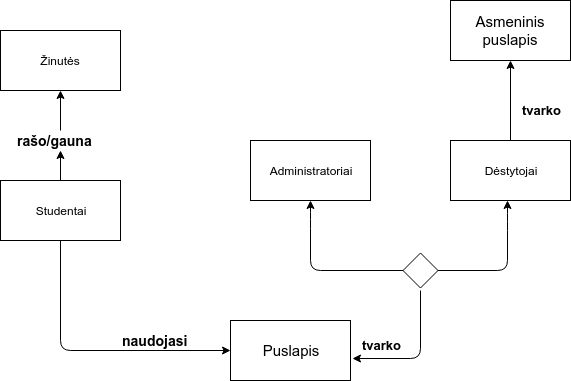
\includegraphics[width=\linewidth]{img/dalykine.png}
	\caption{Dalykinė srities UML diagrama}
	\label{fig:dalykine}
\end{figure}
\ref{fig:dalykine} pav. esybių diagramoje vaizduojamos esybių sąsajos. Pagrindinė esybė Naudotojas,
kuris gali būti Studentas, Dėstytojas arba Administratorius. Studentas turi galimybę naudotis pagrindinėmis puslapio funkcijos, o dėstytojai ir administratoriai pateikti naudingą studentams meždiagą. Taip pat studentai bei dėstytojai gali komunikuoti tarpusavyje nesinaudojant trečiųjų šalių komunikacinėmis priemonėmis. Administratoriai, savo ruožtu, pateikia informaciją apie renginius, naujienas ir D.U.K.
\subsubsection{Klasių diagrama (pirmas lygis)}
\begin{figure}[H]
	\centering
	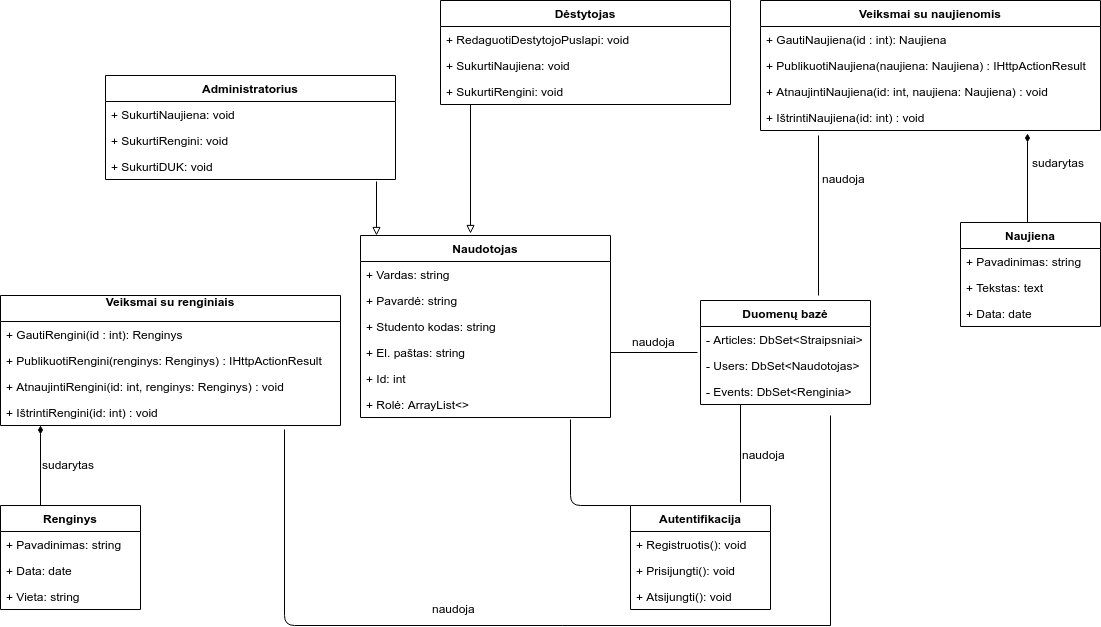
\includegraphics[width=\linewidth]{img/pagrindine.png}
	\caption{Dalykinė srities UML diagrama}
	\label{fig:pagrindine}
\end{figure}
Pagrindinį programos funkcionalumą užtikrina šios klasės: Studentas, Dėstytojas, Administratorius, Reitingas, Dėsytotojo puslapis, Naujienos, Autentifikacija, Duomenų bazė,
D.U.K., Renginiai. Veikimą įgyvendinačių klasių tarpusavio bendradarbiavimas vaizduojamas asociacija, ge-
neralizacija, kompozicija bei kardinalumus (\ref{fig:pagrindine}  pav.).
\newpage
\subsection{UŽDUOČIŲ PJŪVIS}
Šiame skyriuje aprašomas kuriamo socialinio tinklalapio galimi panaudojimo atvejai. Pasinaudojant užduočių diagrama pateikiami studento ir dėstytojo (SocialVU naudotojų) tikslai socialiniam tinklalapiui. Kiekvienai užduočiai pateikiamas scenarijus, kuris parodo, kaip užduotis įgyvendinama.
\subsubsection{Sistemoje vykdomos užduotys}
\begin{figure}[H]
	\centering
	\includegraphics[width=\linewidth]{img/socpslSistema.png}
	\caption{Socialiniame tinklalapyje vykdomos užduotys}
	\label{fig:socpslsist}
\end{figure}
Sistemoje vykdomos pagrindinės užduotys: studentas gali peržiūrėti pasirinkto dėstytojo puslapius. Dėstytojams sudaroma galimybė pateikti aktualias naujienas, informaciją apie renginius, redaguoti savo asmeninius tinklalapius, kuriuose gali talpinti informaciją apie savo dėstomus dalykus bei kitą naudingą informaciją, kurią matys jų studentai. Tiek dėstytojai, tiek studentai gali gauti informaciją apie juos dominančius renginius, matyti aktualias naujienas, gauti bei siųsti žinutes.(\ref{fig:socpslsist} pav.).
\subsubsection{Užduočių vykdymo scenarijai}
Užduočių vykdymo scenarijai, atvaizduoja agentų, šiuo atveju studento ir dėstytojo, įmanomų įvykdyti užduočių veiksmus paeiliui , nuo pradžios iki užduoties vykdymo pabaigos.
\subsubsection{Užduoties "Pridėti naujieną" scenarijus}
\begin{figure}[H]
	\centering
	\includegraphics[scale=0.65]{img/addNew.png}
	\caption{Užduoties "Pridėti naujieną" scenarijus}
	\label{fig:addNew}
\end{figure}
\textbf{Žingsnių seka (\ref{fig:addNew}pav.)}\\
\begin{enumerate}
	\item Sukurti naujieną - dėstytojas paspaudžia ant nuorodos leidžiančios sukurti naujieną.
	\item Informacija apie naujieną? - naujienų UI išmeta dėstytojui naujienos formą užpildymui.
	\item Naujienos informacija - naudotojas išsiunčia užpildytą formą naujienų UI.
	\item Sukurti naujieną - įvesta naujienos informacija yra siunčiama kontroleriui.
	\item Pridėti naujieną - darbų UI įdeda naujieną į duomenų bazę.
	\item Naujiena pridėta - duomenų bazė parsiunčia naujienos patalpinimo patvirtinimą.
	\item Gauti naujienų sąrašą - naujienų kontroleris prašo duomenų bazės pateikti naują naujienų sąrašą.
	\item Naujienų sąrašas - naujienų sąrašas keliauja iš duomenų bazės iki dėstytojo.
\end{enumerate}
\subsubsection{Užduoties "Ištrinti naujieną" scenarijus}
\begin{figure}[H]
	\centering
	\includegraphics[scale=0.65]{img/deleteNew.png}
	\caption{Užduoties "Ištrinti naujieną" scenarijus}
	\label{fig:delNew}
\end{figure}
\textbf{Žingsnių seka (\ref{fig:delNew}pav.)}\\
\begin{enumerate}
	\item Ištrinti naujieną - dėstytojas paspaudžia nuorodą ištrinančią naujieną.
	\item Patvirtinti ištrynimą? - naudotojas prašomas patvirtinti ištrynimą.
	\item Patvirtinti ištrynimą - dėstytojas patvirtina ištrynimą.
	\item Ištrinti naujieną - pateikiama naujiena ištrynimui įvykdyti.
	\item Ištrinti naujieną - prašoma duomenų bazės surasti ir ištrinti naujieną.
	\item Gauti naujienų sąrašą - siunčiamas prašymas naujienų sąrašui gauti iš duomenų bazės.
	\item Naujienų sąrašas - atnaujintas sąrašas keliauja iki dėstytojo.
\end{enumerate}
\subsubsection{Užduoties "Redaguoti naujieną" scenarijus}
\begin{figure}[H]
	\centering
	\includegraphics[scale=0.65]{img/editNew.png}
	\caption{Užduoties "Redaguoti naujieną" scenarijus}
	\label{fig:edNew}
\end{figure}
\textbf{Žingsnių seka (\ref{fig:edNew}pav.)}\\
\begin{enumerate}
	\item Redaguoti naujieną - dėstytojas paspaudžia nuorodą leidžiančią redaguoti naujieną.
	\item Redaguoti naujieną - pateikiama naujiena naujienų kontroleriui.
	\item Surasti naujieną - naujiena ieškoma duomenų bazėje.
	\item Naujiena - duomenų bazė pateikia naujieną kontroleriui.
	\item Naujienos informacija -  informacija apie naujieną keliauja iki naudotojo.
	\item Naujienos informacija - informacija apie naujieną keliauja iki naudotojo.
	\item Išsaugoti pakeitimus - naudotojas prašo išsaugoti įvykdytus pakeitimus.
	\item Redaguoti naujieną - naujiena siunčiama redagavimui.
	\item Išsaugoti pakeitimus - pakeitimai išsaugomi duomenų bazėje.
	\item Gauti naujienų sąrašą - kontroleris prašo duomenų bazės gauti atnaujintą naujienų sąrašą.
	\item Naujienų sąrašas - naujienų sąrašas keliauja iš duomenų bazės iki dėstytojo.
\end{enumerate}
\subsubsection{Užduoties "Peržiūrėti naujienas" scenarijus}
\begin{figure}[H]
	\centering
	\includegraphics[scale=0.65]{img/viewNew.png}
	\caption{Užduoties "Peržiūrėti naujienas" scenarijus}
	\label{fig:viewNew}
\end{figure}
\textbf{Žingsnių seka (\ref{fig:viewNew}pav.)}\\
\begin{enumerate}
	\item Gauti naujienų sąrašą - dėstytojas paspaudžia nuorodą į naujienų sąrašą.
	\item Gauti naujienų sąrašą - prašymas gauti naujienų sąrašą keliauja iki duomenų bazės.
	\item Naujienų sąrašas - naujienų sąrašas iš duomenų bazės keliauja iki naudotojo.
\end{enumerate}
\subsubsection{Užduoties "Pridėti renginį" scenarijus}
\begin{figure}[H]
	\centering
	\includegraphics[scale=0.65]{img/addNewEvent.png}
	\caption{Užduoties "Pridėti renginį" scenarijus}
	\label{fig:addNewEvent}
\end{figure}
\textbf{Žingsnių seka (\ref{fig:addNewEvent}pav.)}\\
\begin{enumerate}
	\item Sukurti renginį - dėstytojas paspaudžia ant nuorodos leidžiančios sukurti renginį.
	\item Informacija apie renginį? - renginių UI išmeta dėstytojui renginio formą užpildymui.
	\item Renginio informacija - naudotojas išsiunčia užpildytą formą renginių UI.
	\item Sukurti renginį - įvesta renginio informacija yra siunčiama kontroleriui.
	\item Pridėti renginį - renginių UI įdeda renginį į duomenų bazę.
	\item Renginys pridėtas - duomenų bazė parsiunčia renginio patalpinimo patvirtinimą.
	\item Gauti renginių sąrašą - renginių kontroleris prašo duomenų bazės pateikti naują renginių sąrašą.
	\item Renginių sąrašas - renginių sąrašas keliauja iš duomenų bazės iki dėstytojo.
\end{enumerate}
\subsubsection{Užduoties "Ištrinti renginį" scenarijus}
\begin{figure}[H]
	\centering
	\includegraphics[scale=0.65]{img/deleteEvent.png}
	\caption{Užduoties "Ištrinti renginį" scenarijus}
	\label{fig:delEvent}
\end{figure}
\textbf{Žingsnių seka (\ref{fig:delEvent}pav.)}\\
\begin{enumerate}
	\item Ištrinti renginį - dėstytojas paspaudžia nuorodą ištrinančią renginį.
	\item Patvirtinti ištrynimą? - naudotojas prašomas patvirtinti ištrynimą.
	\item Patvirtinti ištrynimą - dėstytojas patvirtina ištrynimą.
	\item Ištrinti renginį - pateikiamas renginys ištrynimui įvykdyti.
	\item Ištrinti renginį - prašoma duomenų bazės surasti ir ištrinti renginį.
	\item Gauti renginių sąrašą - siunčiamas prašymas renginių sąrašui gauti iš duomenų bazės.
	\item Renginių sąrašas - atnaujintas sąrašas keliauja iki dėstytojo.
\end{enumerate}
\subsubsection{Užduoties "Redaguoti renginį" scenarijus}
\begin{figure}[H]
	\centering
	\includegraphics[scale=0.65]{img/editEvent.png}
	\caption{Užduoties "Redaguoti renginį" scenarijus}
	\label{fig:editEvent}
\end{figure}
\textbf{Žingsnių seka (\ref{fig:editEvent}pav.)}\\
\begin{enumerate}
	\item Redaguoti renginį - dėstytojas paspaudžia nuorodą leidžiančią redaguoti renginį.
	\item Redaguoti renginį - pateikiamas renginys renginių kontroleriui.
	\item Surasti renginį - renginys ieškomas duomenų bazėje.
	\item Renginys - duomenų bazė pateikia renginį kontroleriui.
	\item Renginio informacija -  informacija apie renginį keliauja iki naudotojo.
	\item Renginio informacija - informacija apie renginį keliauja iki naudotojo.
	\item Išsaugoti pakeitimus - naudotojas prašo išsaugoti įvykdytus pakeitimus.
	\item Redaguoti renginį - renginys siunčiamas redagavimui.
	\item Išsaugoti pakeitimus - pakeitimai išsaugomi duomenų bazėje.
	\item Gauti renginių sąrašą - kontroleris prašo duomenų bazės gauti atnaujintą renginių sąrašą.
	\item Renginių sąrašas - renginių sąrašas keliauja iš duomenų bazės iki dėstytojo.
\end{enumerate}
\subsubsection{Užduoties "Peržiūrėti renginius" scenarijus}
\begin{figure}[H]
	\centering
	\includegraphics[scale=0.65]{img/viewEvent.png}
	\caption{Užduoties "Peržiūrėti renginius" scenarijus}
	\label{fig:viewEvent}
\end{figure}
\textbf{Žingsnių seka (\ref{fig:viewEvent}pav.)}\\
\begin{enumerate}
	\item Gauti renginių sąrašą - dėstytojas paspaudžia nuorodą į renginių sąrašą.
	\item Gauti renginių sąrašą - prašymas gauti renginių sąrašą keliauja iki duomenų bazės.
	\item Renginių sąrašas - renginių sąrašas iš duomenų bazės keliauja iki naudotojo.
\end{enumerate}
\subsubsection{Užduoties "Pridėti D.U.K." scenarijus}
\begin{figure}[H]
	\centering
	\includegraphics[scale=0.65]{img/addDUK.png}
	\caption{Užduoties "Pridėti D.U.K." scenarijus}
	\label{fig:addDuk}
\end{figure}
\textbf{Žingsnių seka (\ref{fig:addDuk}pav.)}\\
\begin{enumerate}
	\item Pridėti D.U.K. - dėstytojas paspaudžia ant nuorodos leidžiančios sukurti D.U.K.
	\item Informacija apie klausimą? - D.U.K. UI išmeta dėstytojui D.U.K. formą užpildymui.
	\item Klausimo informacija - naudotojas išsiunčia užpildytą formą D.U.K. UI.
	\item Sukurti  klausimą - įvesta klausimo informacija yra siunčiama kontroleriui.
	\item Pridėti klausimą - D.U.K. UI įdeda klausimą į duomenų bazę.
	\item Klausimas pridėtas - duomenų bazė parsiunčia klausimo patalpinimo patvirtinimą.
	\item Gauti D.U.K. sąrašą - D.U.K. kontroleris prašo duomenų bazės pateikti naują D.U.K. sąrašą.
	\item D.U.K. sąrašas - D.U.K. sąrašas keliauja iš duomenų bazės iki dėstytojo.
\end{enumerate}
\subsubsection{Užduoties "Peržiūrėti D.U.K." scenarijus}
\begin{figure}[H]
	\centering
	\includegraphics[scale=0.65]{img/viewDUK.png}
	\caption{Užduoties "Peržiūrėti D.U.K." scenarijus}
	\label{fig:viewDUK}
\end{figure}
\textbf{Žingsnių seka (\ref{fig:viewDUK}pav.)}\\
\begin{enumerate}
	\item Gauti D.U.K. sąrašą - dėstytojas paspaudžia nuorodą į D.U.K. sąrašą.
	\item Gauti D.U.K. sąrašą - prašymas gauti D.U.K. sąrašą keliauja iki duomenų bazės.
	\item D.U.K. sąrašas - D.U.K. sąrašas iš duomenų bazės keliauja iki naudotojo.
\end{enumerate}
\subsubsection{Užduoties "Redaguoti pasirinktą klausimą" scenarijus}
\begin{figure}[H]
	\centering
	\includegraphics[scale=0.65]{img/editDUK.png}
	\caption{Užduoties "Redaguoti pasirinktą klausimą" scenarijus}
	\label{fig:editDuk}
\end{figure}
\textbf{Žingsnių seka (\ref{fig:editDuk}pav.)}\\
\begin{enumerate}
	\item Redaguoti pasirinktą klausimą - dėstytojas paspaudžia nuorodą leidžiančią redaguoti klausimą.
	\item Redaguoti pasirinktą klausimą - pateikiamas klausimas D.U.K. kontroleriui.
	\item Surasti pasirinktą klausimą - klausimas ieškomas duomenų bazėje.
	\item Pasirinktas klausimas - duomenų bazė pateikia klausimą kontroleriui.
	\item Klausimo informacija -  informacija apie klausimą keliauja iki naudotojo.
	\item Klausimo informacija - informacija apie klausimą keliauja iki naudotojo.
	\item Išsaugoti pakeitimus - naudotojas prašo išsaugoti įvykdytus pakeitimus.
	\item Redaguoti klausimą - klausimas siunčiamas redagavimui.
	\item Išsaugoti pakeitimus - pakeitimai išsaugomi duomenų bazėje.
	\item Gauti D.U.K. sąrašą - kontroleris prašo duomenų bazės gauti atnaujintą D.U.K. sąrašą.
	\item D.U.K. sąrašas - D.U.K. sąrašas keliauja iš duomenų bazės iki dėstytojo.
\end{enumerate}
\subsubsection{Užduoties "Peržiūrėti pasirinkto dėstytojo teikiamą informaciją" scenarijus}
\begin{figure}[H]
	\centering
	\includegraphics[scale=0.65]{img/viewLecturer.png}
	\caption{Užduoties "Peržiūrėti pasirinkto dėstytojo teikiamą informaciją" scenarijus}
	\label{fig:viewLec}
\end{figure}
\textbf{Žingsnių seka (\ref{fig:viewLec}pav.)}\\
\begin{enumerate}
	\item Gauti dėstytojų sąrašą - studentas paspaudžia nuorodą į dėstytojų sąrašą.
	\item Gauti dėstytojų sąrašą - prašymas gauti dėstytojų sąrašą keliauja iki duomenų bazės.
	\item Gauti dėstytojų sąrašą - prašymas gauti dėstytojų sąrašą keliauja iki duomenų bazės.
	\item Dėstytojų sąrašas - duomenų sąrašas keliauja iki naudotojo.
	\item Dėstytojų sąrašas -  duomenų sąrašas keliauja iki naudotojo.
	\item Pasirinkite dėstytoją - prašoma pasirinkti, kurio dėstytojo puslapį norima matyti.
	\item Pasirinktas dėstytojas - pasirenkamas dėstytojas, kurio informacija domina.
	\item Rodyti tik pasirinktą dėstytoją - dėstytojas siunčiamas kontroleriui.
	\item Surasti pasirinktą dėstytoją -  D.U.K. kontroleris prašo duomenų bazės pateikti dėstytojo puslapį.
	\item Pasirinktas dėstytojas - dėstytojo puslapis keliauja iš duomenų bazės iki studento.
\end{enumerate}
\subsubsection{Užduoties "Peržiūrėti pasirinktą žinutę" scenarijus}
\begin{figure}[H]
	\centering
	\includegraphics[scale=0.65]{img/viewMessage.png}
	\caption{Užduoties "Peržiūrėti pasirinktą žinutę" scenarijus}
	\label{fig:viewMess}
\end{figure}
\textbf{Žingsnių seka (\ref{fig:viewMess}pav.)}\\
\begin{enumerate}
	\item Peržiūrėti žinutes - naudotojas paspaudžia nuorodą peržiūrėti žinutes.
	\item Gauti naudotojo žinutes - prašymas gauti žinutes keliauja iki duomenų bazės.
	\item Gauti naudotojo žinutes - prašymas gauti žinutes keliauja iki duomenų bazės.
	\item Naudotojo žinutės - žinučių sąrašas keliauja iki naudotojo.
	\item Naudotojo žinutės - žinučių sąrašas keliauja iki naudotojo.
	\item Pasirinkite žinutę - leidžiama pasirinkti, kurią žinutę norima matyti.
	\item Pasirinkta žinutė - pasirenkama žinutė, kurios informacija domina.
	\item Rodyti pasirinktos žinutės informaciją - žinutė siunčiama kontroleriui.
	\item Surasti pasirinktą žinutę - Pašto kontroleris prašo duomenų bazės pateikti žinutę.
	\item Pasirinkta žinutė - žinutė keliauja iš duomenų bazės kontroleriui.
	\item Pasirinktos žinutės informacija - žinutė keliauja iš duomenų bazės naudotojui.
\end{enumerate}
\subsubsection{Užduoties "Siųsti žinutę" scenarijus}
\begin{figure}[H]
	\centering
	\includegraphics[scale=0.65]{img/sendMes.png}
	\caption{Užduoties "Siųsti žinutę" scenarijus}
	\label{fig:sendMess}
\end{figure}
\textbf{Žingsnių seka (\ref{fig:sendMess}pav.)}\\
\begin{enumerate}
	\item Siųsti žinutę - naudotojas paspaudžia nuorodą siųsti žinutę.
	\item Informacija apie žinutę - pašto UI išmeta naudotojui žinutės formą užpildymui.
	\item Žinutės informacija - naudotojas suveda žinutės informaciją ir patvirtina siuntimą.
	\item Išsiųsti žinutę - įvesta informacija yra siunčiama kontroleriui.
	\item Pridėti žinutę - pašto UI įdeda žinutę į duomenų bazę.
	\item Žinutė išsiųsta - kontroleris gauna patvirtinimą apie žinutės išsiuntimą.
	\item Gauti naudotojo žinutes - kontroleris prašo duomenų bazės gauti naudotojo žinutes.
	\item Naudotojo žinutės - naudotojo žinučių sąrašas keliauja iš duomenų bazės naudotojui.
\end{enumerate}
\subsubsection{Užduoties "Redaguoti asmeninį dėstytojo puslapį" scenarijus}
\begin{figure}[H]
	\centering
	\includegraphics[scale=0.65]{img/editPage.png}
	\caption{Užduoties  "Redaguoti asmeninį dėstytojo puslapį" scenarijus}
	\label{fig:editPage}
\end{figure}
\textbf{Žingsnių seka (\ref{fig:editPage}pav.)}\\
\begin{enumerate}
	\item Redaguoti asmeninį puslapį - dėstytojas paspaudžia nuorodą redaguoti asmeninį puslapį.
	\item Rodyti dėstytojo puslapį - prašymas rodyti puslapį keliauja į kontrolerį.
	\item Surasti dėstytoją - kontroleris pateikia prašymą duomenų bazei surasti prisijungusį dėstytoją.
	\item Dėstytojo puslapis - rasto dėstytojo puslapio informacija keliauja dėstytojui.
	\item Išsaugoti pakeitimus - atlikęs pakeitimus savo puslapyje, dėstytojas paspaudžia nuorodą išsaugoti.
	\item Redaguoti puslapį - įvesta informacija yra siunčiama kontroleriui.
	\item Išsaugoti pakeitimus - dėstytojo kontroleris įdeda pakeistą informaciją į duomenų bazę.
	\item Rodyti puslapį - kontroleris prašo duomenų bazės gauti redaguotą dėstytojo puslapio informaciją.
	\item Asmeninis dėstytojo puslapis - dėstytojo puslapio informacija keliauja iš duomenų bazės dėstytojui.
\end{enumerate}
\subsubsection{Užduoties "Įkelti konspektą" scenarijus}
\begin{figure}[H]
	\centering
	\includegraphics[scale=0.65]{img/addKons.png}
	\caption{Užduoties  ""Įkelti konspektą" scenarijus}
	\label{fig:addKons}
\end{figure}
\textbf{Žingsnių seka (\ref{fig:addKons}pav.)}\\
\begin{enumerate}
	\item Įkelti konspektą - studentas paspaudžia nuorodą įkelti konspektą.
	\item Informacija apie konspektą, priedas - konspektų UI išmeta studentui konspekto formą užpildymui, bei pasirinkimui failo, kurį norima pridėti.
	\item Konspekto informacija - naudotojas išsiunčia užpildytą formą Konspektų UI.
	\item Įkelti klausimą - pateikta konspekto informacija yra siunčiama kontroleriui.
	\item Pridėti konspektą - Konpektų UI įdeda konspektą į duomenų bazę.
	\item Konspektas pridėtas - duomenų bazė parsiunčia konspekto patalpinimo patvirtinimą.
	\item Gauti konspektų sąrašą - konspektų kontroleris prašo duomenų bazės pateikti naują konspektų sąrašą.
	\item Konspektų sąrašas - Konspektų sąrašas keliauja iš duomenų bazės iki studento.
\end{enumerate}
	\subsubsection{Užduoties "Peržiūrėti konspektus" scenarijus}
	\begin{figure}[H]
		\centering
		\includegraphics[scale=0.65]{img/addKons.png}
		\caption{Užduoties "Peržiūrėti konspektus" scenarijus}
		\label{fig:viewKons}
	\end{figure}
	\textbf{Žingsnių seka (\ref{fig:viewKons}pav.)}\\
	\begin{enumerate}
		\item Gauti konspektų sąrašą - studentas paspaudžia nuorodą į konspektų sąrašą.
		\item Gauti konspektų sąrašą - prašymas gauti konspektų sąrašą keliauja iki duomenų bazės.
		\item Konspektų sąrašas - konspektų sąrašas iš duomenų bazės keliauja iki naudotojo.
	\end{enumerate}
	\newpage
	\subsection{KŪRIMO PJŪVIS}
	Programų sistemos komponentai yra vaizduojami trimis lygmenimis: nuliniu, pirmuoju ir antruoju. Toks komponentų pateikimas leidžia išsamiau apibrėžti sistemos fizinius komponentus, jų konfigūraciją bei tarpusavio ryšius. Komponentų diagramos, atvaizduodamos struktūrą, priklausomybes bei sąsajas, leidžia susidaryti fizinį sistemos vaizdą. Taip pat suteikia galimybę apžvelgti išoriškai matomą komponentų elgseną. Komponentai atvaizduojami naudojant UML komponentų diagramas.
	
	\subsubsection{Komponentų diagramos nulinis lygmuo}
	
	\begin{figure}[H]
		\centering
		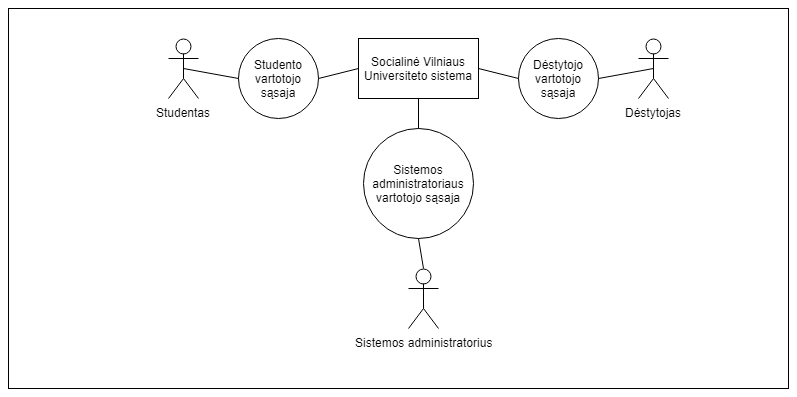
\includegraphics[width=\linewidth]{img/0lygmuo.png}
		\caption{Komponentų diagramos nulinis lygmuo}
		\label{fig:0lygmuo}
	\end{figure}
	
	Komponentų diagramos nuliniame lygmenyje (19 pav.) vaizduojamas bendras komponentų vaizdas. Pagrindinis ir vienintelis šio lygio komponentas yra "Socialinė Vilniaus Universiteto sistema". Šis komponentas sąveikauja su keliomis vartotojo sąsajomis. Studento ir dėstytojo grafinė vartotojo sąsaja įgalina šiuos vartotojus naudotis sistema.
	
	\subsubsection{Komponentų diagramos pirmasis lygmuo}
	
	\begin{figure}[H]
		\centering
		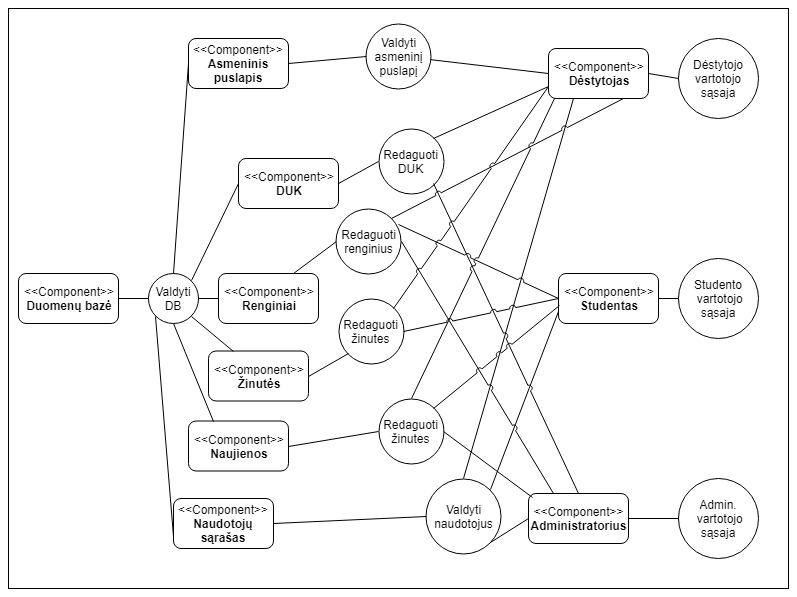
\includegraphics[width=\linewidth]{img/1lygmuo.png}
		\caption{Komponentų diagramos pirmasis lygmuo}
		\label{fig:0lygmuo}
	\end{figure}
	
	Komponentų diagramos pirmame lygmenyje komponentų diagrama yra suskaidoma. Socialinė Vilniaus universiteto sistema yra suskaidoma į šiuos komponentus: Duomenų bazė, Asmeninis puslapis, DUK, Renginiai, Žinutės, Naujienos, Naudotojų sąrašas. Šiame lygyje kiekviena vartotojo sąsaja turi už ją atsakingus komponentus. Taip pat kiekvienas komponentas turi sąsajas su kitais komponentais tam, jog galėtų vykti sąveika ir keitimasis paslaugomis. Tokiu būdu yra užtikrinama visapusiška komponentų realizacija bei tarpusavio darna.
	
	\subsubsection{Komponentų diagramos antrasis lygmuo}
	
	\begin{figure}[H]
		\centering
		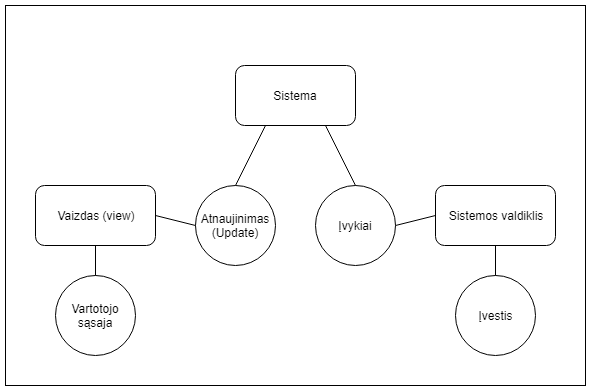
\includegraphics[width=\linewidth]{img/2lygmuo.png}
		\caption{Komponentų diagramos antrasis lygmuo}
		\label{fig:0lygmuo}
	\end{figure}
	
	Antrame lygmenyje dekomponavimui buvo pasitelktas MVC dizaino šablonas. Šis modelis buvo pasirinktas dėl jo paprastumo, universalumo ir populiarumo.
	MVC šabloną sudaro trys pagrindiniai komponentai: Model, View ir Controller. Model (šiuo atveju, mūsų Sistema) – pagrindinis šablono komponentas, jis atsakingas už visos sistemos elgesį probleminėje situacijoje, nepriklausomai nuo vartotojo sąsajos, taip pat jis atsakingas už duomenis, logiką ir taisykles. Vaizdas (view) – komponentas, kuris
	yra atsakingas už informacijos atvaizdavimą, jos atnaujinimą. Valdiklis – komponentas,
	kuris rūpinasi duomenų įvestimi ir įvesties apdorojimu.
	
	\newpage
	\subsection{FIZINIS PJŪVIS}
	Fizinis pjūvis sudarytas iš dislokavimo diagramų. Šiose diagramose vaizduojamas programos komponentų išdėstymas tinkle bei komunikacijos protokolai tarp jų. 
	\subsubsection{Dislokavimo diagrama nr. 1 (komponentų ir artefaktų ryšių diagrama)}
	\begin{figure}[H]
		\centering
		\includegraphics[width=\linewidth]{img/compArtifacts.png}
		\caption{Komponentų ir artefaktų ryšių diagrama}
		\label{fig:compOne}
	\end{figure}
	Komponentų ir artefaktų ryšių diagramoje (\ref{fig:compOne}pav.) vaizduojamas artefaktas SocialVU, kuris įgyvendina šiuos programos komponentus: Autentifikacija, Studentas, Dėstytojas, Naujienų sąrašas, Renginių sąrašas, Žinutės, Asmeninis puslapis.
	\subsubsection{Dislokavimo diagrama nr. 2 (mazgų ir artefaktų ryšių diagrama)}
	\begin{figure}[H]
		\centering
		\includegraphics[width=\linewidth]{img/knotArt.png}
		\caption{Mazgų ir artefaktų ryšių diagrama}
		\label{fig:compTwo}
	\end{figure}
	Mazgų ir artefaktų diagramoje (\ref{fig:compTwo}pav.) parodo, kad tinklalapis yra serveryje, kuris bendrauja hhtp protokolu su SQL serveriu, kuriame saugoma duomenų bazė. Naudotojai turi galimybe pasiekti sistemos teikiamas paslaugas savo pasirinkta naršykle, kuri palaiko http protokolą.
	\subsubsection{Dislokavimo diagrama nr. 3 (mazgų ir artefaktų egzempliorių diagrama)}
	\begin{figure}[H]
		\centering
		\includegraphics[width=\linewidth]{img/knotArtTwo.png}
		\caption{Mazgų ir artefaktų egzempliorių diagrama}
		\label{fig:compThree}
	\end{figure}
	\ref{fig:compThree}pav. vaizduojamas įrenginių (mazgų) išsidėstymas tinkle. Serveris turi tiesioginį ryšį su duomenų baze, o naudotojai gali prisijungti prie serverio. Tačiau nadotojai negali tiesiogiai pasiekti duomenų bazės ir joje saugomų duomenų.
	\newpage
	\subsection{PROCESO PJŪVIS}
	Procesų pjūvis sudarytas iš sekų ir veiklos diagramų. Diagramose parodoma, kokie procesai
	vyksta sistemoje bei išreiškiama komunikacija tarp jų.
	\subsubsection{Proceso sekų diagramos}
	Procesų sekų diagramose, atsispindi procesai, kurie yra vykdomi sistemoje. Iš proceso
	sekų diagramos galima matyti, kokie komponentai dalyvauja vykdyme, kaip procesas vykdomas.
	\begin{figure}[H]
		\centering
		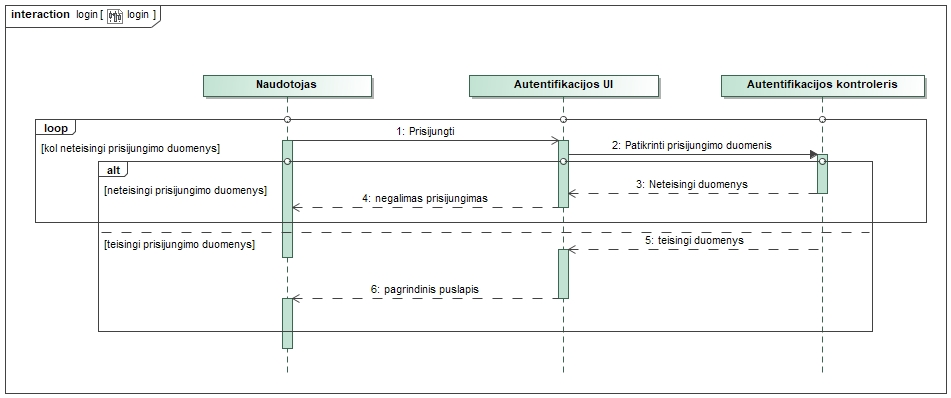
\includegraphics[width=\linewidth]{img/login.jpg}
		\caption{Proceso „Prisijungimas” sekų diagrama}
		\label{fig:login}
	\end{figure}
	Pagal \ref{fig:login} pav. diagramą matoma, kad procesas prasideda naudotojo paspaudimu ant nuorodos įgalinančios prisijungimą. Autentifikacijos
	UI gautus duomenis siunčia patikrinimui į autentifikacijos kontrolerį. Iš kontrolerio
	gaunamas atsakymas, ar duomenys teisingi ar ne. Jei duomenys klaidingi, naudotojui išmetamas pranešimas,
	jog prisijungti negalima ir jis vėl gali kartoti prisijungimo procesą. Jei duomenys teisingi,
	naudotojas yra nukreipiamas į pagrindinį puslapį.
	\begin{figure}[H]
		\centering
		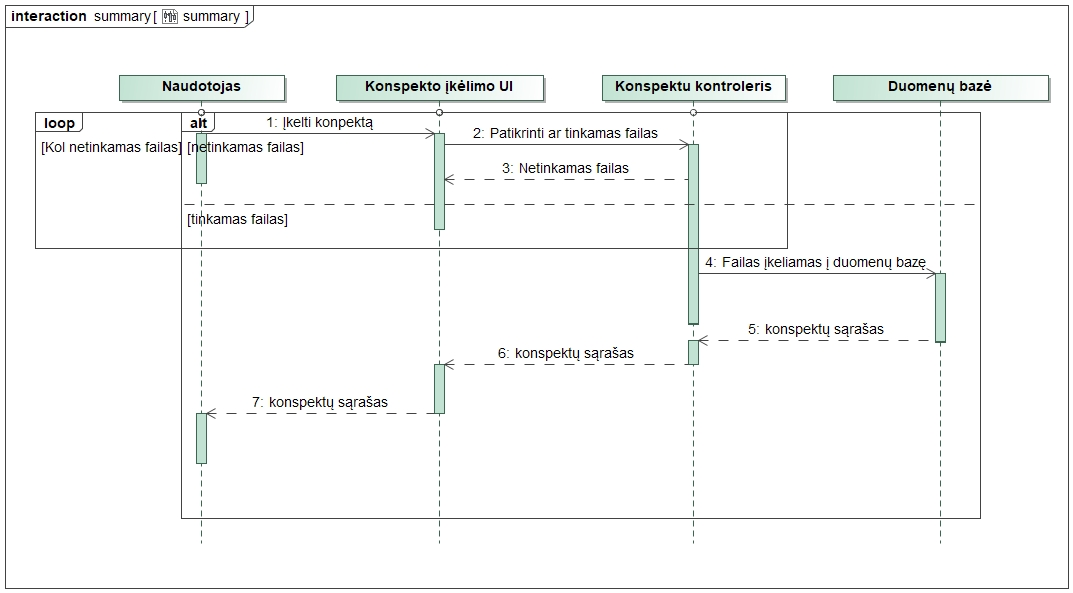
\includegraphics[width=\linewidth]{img/summary.jpg}
		\caption{Proceso „Konspekto įkėlimas” sekų diagrama}
		\label{fig:summary}
	\end{figure}
	Pagal \ref{fig:summary} pav. diagramą matoma, kad procesas prasideda naudotojo paspaudimu ant nuorodos įgalinančios konspekto įkėlimą. Konpekto įkėlimo UI gautus duomenis siunčia patikrinimui į konspektų kontrolerį. Iš kontrolerio
	gaunamas atsakymas, ar failas tinkamas ar ne. Jei failas netinkamas, naudotojui išmetamas pranešimas,
	jog failas netinkamas ir jis vėl gali kartoti konspekto įkėlimo procesą. Jei failas tinkamas, jis yra įkeliamas į duomenų bazę, o
	naudotojas yra nukreipiamas į konspektų puslapį.
	\subsubsection{Veiklos diagramos}
	Veiklos diagramos padeda suprasti dinaminį sistemos
	veikimą, parodo, kokie veiksmai atliekami vykdant konkrečią veiklą, galimus vykdymo atvejus.
	\begin{figure}[H]
		\centering
		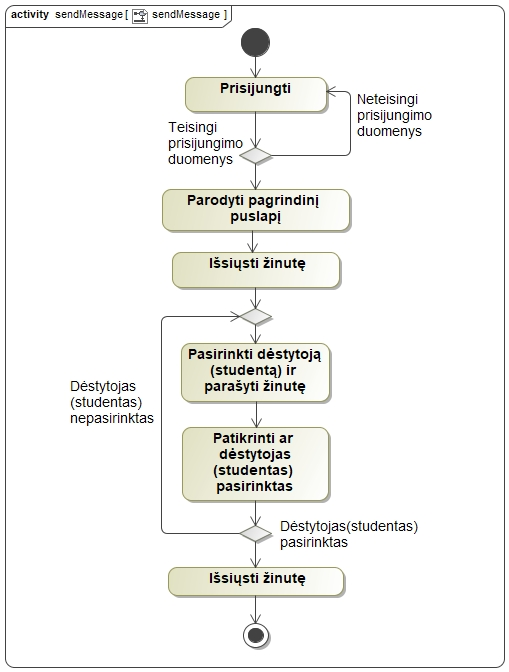
\includegraphics[scale=0.65]{img/sendMessage.jpg}
		\caption{Žinutės išsiuntimo veiklos diagrama}
		\label{fig:sendMessage}
	\end{figure}
	\ref{fig:sendMessage} pav. diagramoje matomas, žinutės išsiuntimo dėstytojui procesas. Procesas prasideda naudotojo
	nuorodos paspaudimu, kreipiančios į žinutės išsiuntimo formą. Naudotojas pateikia parašo žinutę bei pasirenka dėstytoją, tuomet duomenys siunčiami patikrinimui. Jei dėstytojas nebuvo pasirinktas, naudotojas nukreipiamas
	atgal į žinutės siuntimo formą. Jei duomenys atitinka visus reikalavimus, tada žinutė išsiunčiama.
	\begin{figure}[H]
		\centering
		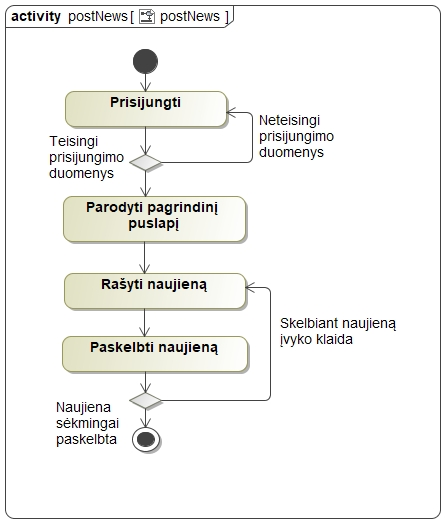
\includegraphics[scale=0.65]{img/postNews.jpg}
		\caption{Naujienos paskelbimo veiklos diagrama}
		\label{fig:postNews}
	\end{figure}
	\ref{fig:postNews} pav. diagramoje matomas, naujienos paskelbimo procesas. Procesas prasideda naudotojo prisijungimu. Neteisingai suvedus prisijungimo duomenis naudotojas vėl nukreipiamas į prisjungimą, kitu atveju jis nukreipiamas į pagridinį puslapį bei pasirenka naujienos paskelbimo nuorodą. Naudotojas parašo naujieną bei ją paskelbia. Jei skelbiant naujieną įvyksta klaida jis nukreipiamas į naujienos rašymo formą, kitu atveju naujiena paskelbiama.
	\newpage
\sectionnonum{REZULTATAI}
Dokumente pateiktas verslo proceso aprašas, kuriamai sistemai atlikta išorinė bei vidinė verslo proceso analizė. Iškelti tikslai, jog sistema naudotųsi bent pusė Vilniaus universiteto studentų. Pateiktos UML diagramos dalykinei sričiai, užduočių veiklai, klasėms.

Atlikus įgyvendinamumo ir naudos analizę paaiškėjo, jog preliminarus metinis sitemos pelnas tūrėtų būti 31284€. atsižvelgiant į sistemos kūrimui ir palaikymui reikalingas išvadas, sistema turėtų tapti pelninga po 1.76 metų.

Pateikti sistemos naudojimo scenarijai. Nurodyti pagrindinių funkcijų modeliai, atvaizduojantys, kaip pagrindiniai sistemos agentai (dėstytojai, studentai bei  administratoriai) naudosis sistema.

Pateikti aiškiai sunumeruoti ir apibrėžti kuriamo socialinio tinklapio funkciniai reikalavimai, o
jų tarpusavio sąveika atvaizduota sekų diagramomis.

Pateikti aiškiai sunumeruoti ir apibrėžti kuriamo socialinio tinklapio funkciniai reikalavimai, o
jų tarpusavio sąveika atvaizduota sekų diagramomis.
Suformuluoti nefunkciniai reikalavimai. Reikalavimai išskirti į šias skiltis: vidinių interfeisų,
veikimo, diegimo, aptarnavimo ir priežiūros, tiražuojamumo, apsaugos bei juridiniai.
Vartotojo sąsajos reikalavimai apibrėžti metaforos reikalavimų lentele bei suformuluotomis užduotimis
įvairiems scenarijams, taip pat pateikiami darnos ir standartizavimo bei pranešimų formulavimo
reikalavimai.

Kuriamos sistemos architektūra išnagrinėta naudojant UML4+1 požiūrių rinkinį. Iš loginio, užduočių, kūrimo, fizinio bei procesų pjūvių matomas sistemos funkcionalumas, užduotys, kurias gali įgyvendinti naudotojas, sąsajos tarp atskirų sistemos komponentų, sistemos įranga bei dinaminis sistemos modelis.

\end{document}